%% ==========================================================================
%%  GAT Virtual Campus -- IEEE journal-style manuscript
%%  Compile with pdfLaTeX on Overleaf (see README.md).
%%  Recommended: pdflatex -> bibtex -> pdflatex -> pdflatex
%% ==========================================================================
\documentclass[journal]{IEEEtran}

% ---- Font encoding (T1 + Latin Modern; keeps <, >, | etc. correct in \texttt) ----
\usepackage[T1]{fontenc}
\usepackage{lmodern}

% ---- Math ----
\usepackage{amsmath,amssymb,amsfonts}
\usepackage{bm}

% ---- Algorithms ----
\usepackage{algorithm}
\usepackage{algpseudocode}

% ---- Float capacity (13 algorithms + 11 figures + 9 tables) ----
\usepackage{morefloats}

% ---- Tables / figures ----
\usepackage{graphicx}
\usepackage{booktabs}
\usepackage{array}
\usepackage{multirow}
\usepackage{makecell}
\usepackage[table]{xcolor}

% ---- Diagrams (editable, self-contained) ----
\usepackage{tikz}
\usetikzlibrary{arrows.meta,positioning,shapes.geometric,calc,fit,backgrounds,decorations.pathreplacing}

% ---- Bibliography / links ----
\usepackage{cite}
\usepackage[hidelinks]{hyperref}
\usepackage{url}

% ---- Convenience macros ----
% \textnormal wrapper keeps the small-caps name upright/medium even inside
% \emph{}, \textbf{}, or IEEEtran's italic subsection headings, so NFSS is
% never asked for the non-existent T1/lmr/bx/sc or T1/lmr/m/scit shapes.
\newcommand{\system}{\textnormal{\textsc{GAT Virtual Campus}}}
\newcommand{\code}[1]{\texttt{#1}}
\newcommand{\kb}{knowledge base}
\newcommand{\etal}{\textit{et al.}}

% IEEEtran algorithm caption spacing
\renewcommand{\algorithmicrequire}{\textbf{Input:}}
\renewcommand{\algorithmicensure}{\textbf{Output:}}

\begin{document}

\title{An Integrated Retrieval-Augmented and Graph-Based Architecture for
Virtual Campus Exploration: Grounded Multi-Agent Question Answering, 360$^{\circ}$
Scene-Graph Navigation, and A$^{\star}$ Wayfinding}

\author{
        Author~One,
        Author~Two,
        and~Author~Three% <-- replace with real authors
\thanks{Manuscript prepared \today. \emph{(Corresponding author: Author One.)}}
\thanks{The authors are with the Department of Computer Science and
Engineering, Global Academy of Technology, Bengaluru 560098, India
(e-mail: author.one@example.com; author.two@example.com;
author.three@example.com).}
\thanks{Source code and reproduction artifacts for the implemented system are
maintained in the project repository. This manuscript documents the system
as implemented; components that are partially implemented, unused, or
proposed for future evaluation are labeled as such throughout.}
}

\markboth{IEEE Transactions (Preprint), Vol.~XX, No.~X, Month~2026}%
{Author \MakeLowercase{\textit{et al.}}: An Integrated RAG and Graph-Based Architecture for Virtual Campus Exploration}

\maketitle

\begin{abstract}
Prospective students, parents, and visitors of a university campus face two
distinct information problems: understanding \emph{what} the institution
offers (admissions, programs, facilities, regulations) and understanding
\emph{where} things are on a campus they may never have physically visited.
Existing digital solutions typically address only one of these needs, and
conversational solutions built on large language models (LLMs) are prone to
fabricating institution-specific facts. This paper presents \system{}, a
full-stack platform that integrates a grounded retrieval-augmented
generation (RAG) assistant, a graph-structured 360$^{\circ}$ virtual tour,
and a database-backed A$^{\star}$ wayfinding engine into a single
application built on Next.js, FastAPI, PostgreSQL, ChromaDB, and a locally
hosted Llama~3.2 model served through Ollama. We describe, with reference to
the implemented source code, thirteen algorithmic components: a hybrid
dense--lexical retriever that fuses \code{all-MiniLM-L6-v2} cosine
similarity and BM25 with a $0.6/0.4$ weighting over min--max normalized
scores; a deterministic four-feature reranker; a two-term
intent/retrieval confidence estimator that gates generation; a
post-generation numeric-claim verification pass; a deterministic-first,
LSTM-fallback multi-agent router with five specialist agents; a
per-floor doubly linked list panorama scene graph with a tail-to-head
cross-floor stitching pass; a six-phase guided-tour traversal automaton;
an SVG minimap projection; and an A$^{\star}$ search whose heuristic
degrades gracefully from planar coordinates to a great-circle
approximation to zero (pure Dijkstra). We report implementation-scale
measurements: a $1{,}507$-chunk knowledge base derived from $128$ official
institutional PDFs and $42$ website pages, a $180$-node/$325$-edge campus
graph, $161$ panorama scenes across five floors, and a PyTorch LSTM intent
classifier trained on $168$ synthetic examples across $12$ classes
(training accuracy $1.00$, held-out validation accuracy $0.529$). We are
explicit that no formal retrieval-quality, answer-faithfulness, or
user-study evaluation has yet been performed; the paper therefore
contributes a system-level architecture, a detailed algorithmic
description, and a rigorous proposed evaluation protocol rather than
experimental performance claims.

\end{abstract}

\begin{IEEEkeywords}
Retrieval-augmented generation, virtual campus, 360$^{\circ}$ virtual tour,
multi-agent systems, hybrid information retrieval, BM25, dense retrieval,
sentence embeddings, A$^{\star}$ pathfinding, intent classification, large
language models, grounded generation, hallucination mitigation, campus
navigation, conversational assistant.
\end{IEEEkeywords}

\section{Introduction}
\IEEEPARstart{T}{he} decision to enrol at a particular engineering college
is made, in large part, before the applicant ever sets foot on the campus.
Prospective students and their families gather information from institutional
websites, PDF brochures, ranking portals, and word of mouth, and they form
a mental model of the campus --- its departments, laboratories, hostel,
library, transport, and physical layout --- from fragmentary and often
inconsistent sources. Two information needs dominate this process. The
first is \emph{propositional}: what are the admission routes, the eligibility
criteria, the fee structure, the programs on offer, the accreditation
status? The second is \emph{spatial}: where is the Computer Science block,
which floor is a given laboratory on, what does the central quadrangle
actually look like, and how would one walk from the main gate to the
auditorium?

Digital campus experiences typically serve one of these needs well and the
other poorly. Institutional websites and chatbots answer propositional
questions but present the campus as a list of building names. Virtual-tour
products render 360$^{\circ}$ imagery but carry no queryable knowledge and
no notion of a route. Interactive campus maps show geography but not the
institution's policies or its interiors. A visitor who wants to know
\emph{``which floor is the Power System Simulation Lab on, and can I see
it?''} is served by neither category alone.

At the same time, the natural technology for a unified conversational
interface --- a large language model (LLM) --- introduces a well-documented
failure mode. LLMs asked institution-specific questions readily produce
fluent but fabricated answers: invented faculty names, wrong phone numbers,
plausible-sounding but incorrect fee figures~\cite{ji2023hallucination}.
For a system whose entire value proposition is being an authoritative
substitute for the official sources, an ungrounded answer is worse than no
answer. Retrieval-augmented generation (RAG)~\cite{lewis2020rag} mitigates
this by conditioning the model on retrieved evidence, but a naive RAG
pipeline still hallucinates when retrieval is weak, when the evidence is
thin, or when the model over-extrapolates from a partially relevant
passage~\cite{shuster2021retrieval,gao2023ragsurvey}.

\subsection{The \system{} System}
This paper describes \system{}, an integrated platform developed for the
Global Academy of Technology (GAT), Bengaluru, that combines the
propositional and spatial modalities in a single web application and treats
groundedness as a first-class engineering requirement. The system comprises
three cooperating subsystems:

\begin{enumerate}
\item A \textbf{grounded RAG assistant} that answers natural-language
questions using a knowledge base built exclusively from official
institutional sources ($128$ PDFs and $42$ web pages, $1{,}507$ text
chunks). Retrieval is hybrid (dense embeddings plus BM25); generation is
performed by a locally hosted Llama~3.2 model constrained by a
grounding-only system prompt, a confidence gate that can refuse before the
model is ever called, and a post-generation verification pass that
withholds answers containing unverifiable numeric or contact details.
\item A \textbf{360$^{\circ}$ virtual tour} of the institution's main
building, structured as a per-floor doubly linked list of panorama scenes
with graph-derived branch connections and a construction pass that stitches
floor boundaries so that both manual and automatic (``guided'') traversal
cross between floors with no floor-boundary-specific code.
\item A \textbf{campus navigation engine} implementing A$^{\star}$ shortest
paths over a $180$-node, $325$-edge graph that is rebuilt on demand from
the live PostgreSQL relational schema, with a heuristic that adapts to the
coordinate information actually available for each node pair.
\end{enumerate}

Query routing between the RAG assistant's specialist agents is performed by
a deterministic phrase- and keyword-matching supervisor, with a small
trained LSTM intent classifier consulted only as a fallback for phrasings
the deterministic rules do not cover. Voice input is provided through the
browser-native Web Speech API and feeds the same text pipeline as typed
input.

\subsection{Contributions}
This work makes the following contributions, stated conservatively and
tied directly to the implemented artifact:

\begin{enumerate}
\item A \textbf{system-level architecture} that unifies grounded
conversational question answering, 360$^{\circ}$ scene-graph tour
navigation, and graph-based wayfinding for a single institution, with all
three subsystems sharing one relational campus model and one web/service
stack (Section~\ref{sec:architecture}).
\item A detailed, \textbf{code-verified algorithmic description} of a
layered hallucination-mitigation design for institutional RAG: query
expansion for candidate generation, weighted dense--lexical score fusion,
a deterministic reranker, a two-term confidence gate, a grounding-only
prompt, and an independent post-generation numeric-claim check
(Section~\ref{sec:rag}, Algorithms~\ref{alg:kb}--\ref{alg:grounding}).
\item A \textbf{deterministic-primary, ML-fallback multi-agent routing}
scheme with full decision logging, and an honest account of a trained
LSTM intent classifier integrated as a subordinate signal rather than the
primary router (Section~\ref{sec:agents},
Algorithms~\ref{alg:routing}--\ref{alg:lstm}).
\item A \textbf{doubly-linked-list panorama scene graph} with a
tail-to-head cross-floor stitching mechanism that renders floor-boundary
traversal transparent to every consumer, and a six-phase guided-tour
traversal automaton with cancellation-token and cycle-guard safety
(Section~\ref{sec:tour}, Algorithms~\ref{alg:tourwalk}--\ref{alg:guided}).
\item A \textbf{database-backed A$^{\star}$ wayfinding engine} with a
three-tier degrading heuristic, together with a graph-construction
procedure that treats a normalized relational schema as the live source of
truth for the navigation graph (Section~\ref{sec:nav},
Algorithms~\ref{alg:graphbuild}--\ref{alg:astar}).
\item A set of \textbf{verified implementation-scale measurements} and a
\textbf{proposed evaluation protocol} (Section~\ref{sec:eval}) covering
retrieval quality, reranker ablation, intent-classifier generalization,
answer faithfulness, confidence-threshold calibration, pathfinding
performance, and usability --- experiments that the current artifact does
not yet include and that this paper does not pre-empt with fabricated
numbers.
\end{enumerate}

\subsection{Scope and Honesty Statement}
Consistent with reproducible-systems practice, we distinguish throughout
between (a)~what is implemented, (b)~what has been measured, (c)~what is
proposed for evaluation, and (d)~what is future work. Several components are
partial: the support-vector reranker is implemented but never trained and
is not the production path; the LSTM classifier's probability is not yet
wired into the confidence estimator; the A$^{\star}$ engine has no
front-end consumer; and a previously built three-dimensional map and
GPS turn-by-turn interface were deliberately removed from the codebase.
These facts are reported where relevant rather than elided.

The remainder of the paper is organized as follows.
Section~\ref{sec:related} surveys related work across ten areas and
positions \system{} against it. Section~\ref{sec:problem} formalizes the
problem and objectives. Section~\ref{sec:architecture} presents the system
architecture. Sections~\ref{sec:dataset}--\ref{sec:nav} detail the campus
knowledge representation, the virtual tour engine, the RAG pipeline, the
multi-agent and intent-classification subsystem, and the navigation engine.
Section~\ref{sec:voice} covers voice interaction and
Section~\ref{sec:impl} the implementation and technology stack.
Section~\ref{sec:eval} defines the proposed experimental methodology;
Section~\ref{sec:results} reports the measurements that currently exist and
discusses them. Sections~\ref{sec:limitations}--\ref{sec:conclusion} give
limitations, future work, and conclusions.

\section{Related Work and Literature Survey}
\label{sec:related}
\system{} sits at the intersection of ten research areas. We review each,
identify representative methods, their strengths and limitations, and how
the implemented architecture relates to them. Table~\ref{tab:comparison}
consolidates the comparison against representative campus-oriented and
RAG-oriented systems.

\subsection{Retrieval-Augmented Generation}
RAG~\cite{lewis2020rag} conditions a generative model on passages retrieved
from a non-parametric memory, improving factuality on knowledge-intensive
tasks and allowing the knowledge store to be updated without retraining.
The now-standard pipeline --- chunk a corpus, embed the chunks, retrieve
top-$k$ by vector similarity, and prompt an LLM with the concatenated
passages --- is surveyed comprehensively by Gao~\etal~\cite{gao2023ragsurvey},
who taxonomize \emph{naive}, \emph{advanced}, and \emph{modular} RAG and
catalogue the failure points: retrieval misses, low-precision context,
context-conflict, and over-generation beyond the evidence. Shuster
\etal~\cite{shuster2021retrieval} show that retrieval augmentation
measurably reduces hallucination in dialogue but does not eliminate it,
motivating additional grounding safeguards. Agentic variants such as
ReAct~\cite{yao2023react} interleave retrieval with reasoning steps.

\emph{Relation to \system{}.} The implemented pipeline is ``advanced RAG''
in Gao~\etal's taxonomy: it adds pre-retrieval query expansion, a
post-retrieval reranking and context-selection stage, a confidence gate,
and a post-generation verification stage around the core retrieve-then-read
loop. It is deliberately \emph{not} agentic in the ReAct sense --- the LLM
is never given tools or a multi-step scratchpad --- because the target
deployment is a low-resource, CPU-only local model where each generation
call costs several seconds and predictable single-shot latency was judged
more important than iterative refinement.

\subsection{Dense Retrieval and Sentence Embeddings}
Dense passage retrieval (DPR)~\cite{karpukhin2020dpr} trains a dual-encoder
to embed queries and passages into a shared space where relevance is inner
product, outperforming BM25 on open-domain QA when in-domain training data
is available. Sentence-BERT~\cite{reimers2019sbert} makes such embeddings
practical for unsupervised semantic similarity by fine-tuning
BERT~\cite{devlin2019bert} --- itself a Transformer
encoder~\cite{vaswani2017attention} --- with a siamese objective. Earlier
static embeddings~\cite{mikolov2013word2vec,pennington2014glove} lacked the
contextualization such tasks need. The widely used \code{all-MiniLM-L6-v2}
model combines the Sentence-BERT recipe with the MiniLM distillation of
Wang~\etal~\cite{wang2020minilm} to yield a 384-dimensional encoder small
enough to run on commodity CPUs.
Late-interaction models such as ColBERT~\cite{khattab2020colbert} retain
token-level detail at higher index cost. Approximate nearest-neighbor
indexes --- HNSW~\cite{malkov2020hnsw}, the graph structure used by the
ChromaDB store in this work, and IVF/PQ methods~\cite{johnson2019faiss} ---
make vector search scale.

\emph{Relation to \system{}.} Dense retrieval is used as an
\emph{adopted component}, not a contribution: the pretrained
\code{all-MiniLM-L6-v2} encoder is run locally with L2-normalized
embeddings and cosine ANN search over an HNSW-indexed ChromaDB collection.
No fine-tuning is performed, because no in-domain (query, passage) relevance
data exists for this institution.

\subsection{Lexical Retrieval and BM25}
The probabilistic relevance framework and its BM25 instantiation
\cite{robertson1994okapi,robertson2009bm25} remain the strongest
unsupervised sparse baseline. BM25 scores a document by a saturating
term-frequency function, an inverse-document-frequency weight derived from
Sp\"arck~Jones's term-specificity argument~\cite{sparckjones1972idf}, and a
length-normalization term controlled by parameters $k_1$ and $b$
\cite{manning2008ir}. Its strength is exact-term precision --- it never
confuses ``CSE'' with ``ECE'' the way a smooth embedding space can --- and
its weakness is vocabulary mismatch: a paraphrased query with no shared
terms retrieves nothing.

\emph{Relation to \system{}.} BM25 (the Okapi variant, \code{rank\_bm25})
is indexed over the same chunk set as the dense store, with a deliberately
minimal lowercase-alphanumeric tokenizer and no stemming or stop-word
removal, so that acronyms, department codes, and room numbers survive
intact. It is one of two retrieval signals, never used alone.

\subsection{Hybrid Retrieval and Reranking}
Combining dense and sparse signals consistently beats either alone
\cite{wang2021interpolation}. Fusion can be score-level (weighted sums of
normalized scores) or rank-level (reciprocal rank fusion,
RRF~\cite{cormack2009rrf}); Bruch~\etal~\cite{bruch2023fusion} analyze
convex combinations and show that normalization choice matters more than
the exact weight. A second stage typically reranks a shortlist with a
cross-encoder~\cite{nogueira2019bertrerank} or a sequence-to-sequence
model~\cite{nogueira2020monot5}, trading latency for precision; learning-
to-rank with support-vector regression~\cite{smola2004svr} is a lighter
alternative when labeled relevance judgments exist.

\emph{Relation to \system{}.} The implemented fusion is a convex score-level
combination ($0.6$ dense, $0.4$ lexical) over per-method min--max
normalized candidate sets, consistent with Bruch~\etal's finding that
per-method normalization is what makes a fixed weight meaningful. The
second stage is a \emph{deterministic four-feature weighted sum}, not a
neural cross-encoder, chosen for explainability and zero added model cost.
A support-vector reranker is implemented behind the same interface but is
\emph{never trained} for lack of relevance labels, and is reported as an
unevaluated extension point rather than a result.

\subsection{Hallucination Mitigation and Grounded Generation}
Ji~\etal~\cite{ji2023hallucination} survey intrinsic and extrinsic
hallucination and the mitigation families: faithful decoding, retrieval
grounding, and post-hoc verification. Post-hoc approaches include
SelfCheckGPT~\cite{manakul2023selfcheckgpt}, which samples multiple
generations and checks consistency, and FActScore~\cite{min2023factscore},
which decomposes a generation into atomic facts and verifies each against a
knowledge source. RAGAS~\cite{es2024ragas} operationalizes
\emph{faithfulness}, \emph{answer relevancy}, and \emph{context relevancy}
as LLM-judged metrics for RAG systems.

\emph{Relation to \system{}.} The implemented design layers four
independent safeguards: (i)~retrieval grounding; (ii)~a grounding-only
system prompt with explicit negative instructions; (iii)~a confidence gate
that returns a fixed refusal string \emph{without invoking the LLM} when
the retrieval-quality signal is low; and (iv)~a deterministic
post-generation pass that extracts phone-number, currency, room-number, and
year patterns from the generated answer, reduces each to a digit sequence,
and withholds the whole answer if any such sequence is absent from the
retrieved context. This last check is narrower than FActScore (it targets
checkable numeric claims, not arbitrary sentences) but requires no
additional model call --- an appropriate trade-off for a local-inference
deployment. Formal faithfulness measurement in the style of RAGAS is
proposed but not yet performed (Section~\ref{sec:eval}).

\subsection{Multi-Agent Systems and Query Routing}
The multi-agent paradigm~\cite{wooldridge2009mas} decomposes a task across
specialized agents coordinated by a supervisor or a shared protocol. LLM-
based instantiations --- AutoGen~\cite{wu2023autogen},
MetaGPT~\cite{hong2024metagpt}, HuggingGPT~\cite{shen2023hugginggpt}, and
generative agents~\cite{park2023generative} --- use an LLM both to route
and to execute, which is powerful but expensive and hard to audit. Intent-
based routing, by contrast, classifies the query once and dispatches to a
handler; the classifier can be rule-based, a shallow neural model, or an
LLM.

\emph{Relation to \system{}.} The router is a \emph{deterministic}
phrase- and keyword-matching supervisor: a $23$-entry navigation-phrase
list, a bare-room-number regular expression, and four domain keyword sets
are checked in order, and a trained LSTM intent classifier is consulted
\emph{only} when no deterministic rule fires. Every routing decision is a
literal substring match logged with its trigger, satisfying an explicit
auditability requirement. This is a design choice against the LLM-router
trend, motivated by predictability, zero routing latency, and the ability
to explain any decision post hoc. A lightweight ``multi-domain'' path
splits conjunctive queries into clauses and dispatches each independently.

\subsection{Intent Classification with Recurrent Models}
Spoken-language-understanding research established RNN-based joint intent
detection and slot filling on corpora such as ATIS~\cite{hemphill1990atis}
and SNIPS~\cite{coucke2018snips}; attention-augmented
bi-LSTMs~\cite{liu2016attention} and later BERT-based
classifiers~\cite{chen2019bertintent} are the standard baselines. LSTMs
\cite{hochreiter1997lstm} remain a reasonable choice for short-utterance
classification when training data is scarce and inference must be cheap,
though small datasets invite overfitting~\cite{goodfellow2016deep}. Open
instruction-tuned LLMs~\cite{touvron2023llama2,grattafiori2024llama3} are
an alternative zero-shot classifier but incur per-query inference cost.

\emph{Relation to \system{}.} The implemented classifier is an
\code{embedding}$\rightarrow$\code{LSTM}$\rightarrow$\code{dropout}$\rightarrow$\code{linear}
network with $32$-dimensional embeddings and hidden state, trained on
$168$ hand-authored synthetic utterances across $12$ intent classes. Its
measured held-out accuracy ($0.529$, against a training accuracy of
$1.00$) is characteristic of overfitting on a tiny synthetic set; we
therefore use it strictly as a \emph{fallback signal} behind the
deterministic rules and report its confusion matrix honestly
(Section~\ref{sec:results}).

\subsection{Virtual Tours and 360$^{\circ}$ Panoramic Navigation}
Immersive 360$^{\circ}$ tours are widely used in cultural heritage and
real estate~\cite{argyriou2020360design}, and hyperlinked panoramic video
navigation~\cite{neng2010hypervideo} predates them. The dominant
consumer reference is Google Street View~\cite{anguelov2010streetview},
which models the world as a graph of panoramas connected by navigable
links and preserves camera heading across transitions to maintain a sense
of continuous motion. Web viewers such as
Pannellum~\cite{petroff2019pannellum} render equirectangular imagery in the
browser.

\emph{Relation to \system{}.} The tour is a Street-View-style panorama
graph, but with an explicit data-structure contribution: each floor is a
\emph{doubly linked list} of scene nodes (enabling $O(1)$ sequential
traversal and ``scene $x$ of $y$'' counting scoped to a floor), branch and
vertical connections are held as separate cross-reference pointers, and a
dedicated construction pass links each floor's tail node to the next
floor's head node so that sequential traversal --- manual or automatic ---
crosses floor boundaries with no boundary-aware code. Entry heading is
carried on each link, Street-View style.

\subsection{Indoor Navigation, Wayfinding, and A$^{\star}$}
Indoor navigation systems~\cite{fallah2013indoor} combine a localization
technology~\cite{zafari2019localization} with a routing algorithm over a
navigation graph. The routing algorithm is almost always
Dijkstra's~\cite{dijkstra1959note} or its informed generalization
A$^{\star}$~\cite{hart1968astar}, which expands nodes in order of
$f(n)=g(n)+h(n)$ and is optimal when the heuristic $h$ is admissible
\cite{russell2020aima}.

\emph{Relation to \system{}.} The engine implements A$^{\star}$ with a
binary heap over an adjacency-list graph built on demand from the
relational schema. Its heuristic degrades in three tiers --- Euclidean
distance on planar floor-plan coordinates, an equirectangular great-circle
approximation on latitude/longitude, or zero --- and at the zero tier the
search is provably equivalent to Dijkstra's, which is used directly for
single-source nearest-facility queries. Localization is out of scope: the
endpoint consumes graph node identifiers, and mapping a physical position
to a node is left to the client.

\subsection{Conversational AI for Educational Institutions}
Systematic reviews of educational chatbots
\cite{okonkwo2021chatbots,perez2020chatbots,winkler2018chatbots} report
that most deployed systems are intent-and-response or FAQ retrieval
systems, that admissions and student-services queries dominate real usage,
and that trust and answer correctness are the principal barriers to
adoption. Few reported systems combine a conversational assistant with
spatial exploration of the same campus.

\emph{Relation to \system{}.} \system{} targets exactly the
admissions/academics/facilities query mix these reviews identify, but
replaces the FAQ-retrieval or scripted-intent backend with grounded RAG
over the institution's own documents, and couples it to a spatial tour and
a wayfinding graph of the same campus --- the integration that the reviews
find largely absent.

\begin{table*}[!t]
\centering
\caption{Positioning of \system{} Against Representative Campus-Oriented and RAG-Oriented Systems.
Entries describe \emph{category} characteristics; \system{} entries describe the \emph{implemented} artifact.}
\label{tab:comparison}
\footnotesize
\renewcommand{\arraystretch}{1.25}
\begin{tabular}{@{}p{2.7cm}p{2.1cm}p{2.0cm}p{1.9cm}p{1.6cm}p{1.7cm}p{3.0cm}@{}}
\toprule
\textbf{System class} & \textbf{Info.\ retrieval} & \textbf{Generation / QA} & \textbf{Multi-agent routing} & \textbf{360$^{\circ}$ tour} & \textbf{Graph wayfinding} & \textbf{Principal limitation} \\
\midrule
Institutional website + scripted chatbot &
Keyword / FAQ match &
Templated / canned &
No &
No &
No &
No paraphrase robustness; no spatial context \\

Educational FAQ chatbot \cite{okonkwo2021chatbots,perez2020chatbots} &
Intent + slot &
Retrieval of stored answers &
Intent classifier only &
No &
No &
Answer set is fixed; brittle to unseen intents \\

Naive RAG assistant \cite{lewis2020rag,gao2023ragsurvey} &
Dense top-$k$ &
LLM over concatenated passages &
No &
No &
No &
Hallucinates on weak/thin retrieval; no refusal \\

Agentic RAG (ReAct-style) \cite{yao2023react,wu2023autogen} &
Iterative dense &
LLM with tool loop &
LLM-as-router &
No &
No &
High latency; routing not auditable; cost \\

360$^{\circ}$ virtual tour product \cite{argyriou2020360design,petroff2019pannellum} &
None &
None &
No &
Yes (scenes + hotspots) &
No &
No queryable knowledge; no routes \\

Street View-style panorama graph \cite{anguelov2010streetview} &
None &
None &
No &
Yes (panorama graph) &
Partial (link graph) &
Outdoor scale; no institutional knowledge \\

Indoor navigation system \cite{fallah2013indoor,zafari2019localization} &
None &
None &
No &
No &
Yes (Dijkstra / A$^{\star}$) &
Requires a localization technology; no QA \\

\midrule
\textbf{\system{} (this work)} &
\textbf{Hybrid dense + BM25, $0.6/0.4$ fusion, 4-feature rerank} &
\textbf{Local Llama~3.2, grounding-only prompt, confidence gate + post-hoc numeric check} &
\textbf{Deterministic phrase/keyword first; LSTM fallback; logged} &
\textbf{Yes: per-floor doubly linked list, cross-floor stitching, guided walk} &
\textbf{Yes: A$^{\star}$ over live relational graph, 3-tier heuristic} &
\textbf{No formal evaluation yet; A$^{\star}$ has no front-end; SVR reranker untrained} \\
\bottomrule
\end{tabular}
\end{table*}


\section{Problem Formulation and Research Objectives}
\label{sec:problem}

\subsection{Problem Statement}
Let $\mathcal{D}$ be the set of authoritative documents an institution
publishes about itself (web pages, PDF brochures, regulations), and let
$\mathcal{G}=(V,E)$ be a graph model of its physical campus in which
vertices $V$ are navigable points (entrances, junctions, corridors, rooms,
staircases, landmarks) and edges $E$ are walkable connections with
traversal costs. Let $\mathcal{P}$ be a set of 360$^{\circ}$ panoramic
images, each associated with a vertex $v\in V$.

A user issues either a natural-language query $q$ or a spatial request
$(v_s, v_g)$. The system must:

\begin{itemize}
\item \textbf{P1 (grounded answering).} For a query $q$, return an answer
$a$ together with a set of provenance references $S\subseteq\mathcal{D}$
such that every verifiable claim in $a$ is entailed by
$\bigcup_{s\in S}\mathrm{text}(s)$, \emph{or} return an explicit refusal
when $\mathcal{D}$ does not adequately support an answer. The system must
prefer refusal to an unsupported answer.
\item \textbf{P2 (routing).} Assign $q$ to the specialist handler(s) whose
domain it belongs to, deterministically and explainably where possible.
\item \textbf{P3 (wayfinding).} For $(v_s,v_g)$, return a minimum-cost walk
$\pi = (v_s,\dots,v_g)$ in $\mathcal{G}$, its total cost, an estimated
walking time, an accessibility flag, and human-readable turn-by-turn
directions.
\item \textbf{P4 (tour traversal).} Support both manual step-by-step and
automatic sequential traversal of $\mathcal{P}$ along $\mathcal{G}$,
including transitions between floors, while preserving camera-heading
continuity.
\item \textbf{P5 (integration).} Serve P1--P4 from one application over one
shared campus model, deployable on commodity hardware with no external
paid API.
\end{itemize}

\subsection{Design Constraints}
The implemented system operates under constraints that shape every
subsequent design decision:

\begin{enumerate}
\item \emph{No external LLM API.} All generation and embedding runs locally
(Ollama-served Llama~3.2; \code{all-MiniLM-L6-v2}). This bounds model
capability and makes each generation call cost several seconds of CPU time.
\item \emph{Authoritative sources only.} The knowledge base is built
exclusively from the institution's own domain; third-party aggregators,
encyclopedias, and search snippets are excluded by policy.
\item \emph{Groundedness over coverage.} A wrong answer is a more serious
failure than a refusal, because the system's purpose is to be a trustworthy
substitute for the official sources.
\item \emph{Auditability.} Routing decisions and low-confidence refusals
must be explainable after the fact from logs.
\item \emph{Placeholder-to-real asset path.} Panorama imagery and surveyed
coordinates are placeholders; the code must accept real assets by
file/identifier substitution without logic changes.
\end{enumerate}

\subsection{Research Objectives}
\begin{description}
\item[O1] Design and implement a hybrid retrieval pipeline that combines
semantic and exact-term matching for an acronym- and number-heavy
institutional corpus (Section~\ref{sec:rag}).
\item[O2] Design a layered generation-time safety mechanism --- confidence
gating plus post-hoc claim verification --- that reduces the risk of
unsupported institutional claims without a second model call
(Section~\ref{sec:rag}).
\item[O3] Design a routing mechanism that is deterministic and auditable
for covered phrasings and gracefully falls back to a learned classifier for
uncovered ones (Section~\ref{sec:agents}).
\item[O4] Design a scene-graph data structure for 360$^{\circ}$ tour
navigation that makes cross-floor traversal transparent to traversal code
(Section~\ref{sec:tour}).
\item[O5] Implement graph-based wayfinding whose heuristic adapts to
whatever spatial information is available and remains correct in all cases
(Section~\ref{sec:nav}).
\item[O6] Define a rigorous evaluation protocol for all of the above, and
report honestly the measurements that currently exist
(Sections~\ref{sec:eval}--\ref{sec:results}).
\end{description}

\subsection{Non-Goals}
The following are explicitly out of scope for the implemented artifact:
real-time indoor localization; outdoor GPS turn-by-turn guidance (a
prototype was built and then removed); automatic translation of retrieved
evidence (the assistant answers in the user's selected language via the
LLM, but retrieval remains English); authentication and multi-tenant
isolation; and streaming token-by-token responses.

\section{System Architecture}
\label{sec:architecture}
\begin{figure*}[!t]
\centering
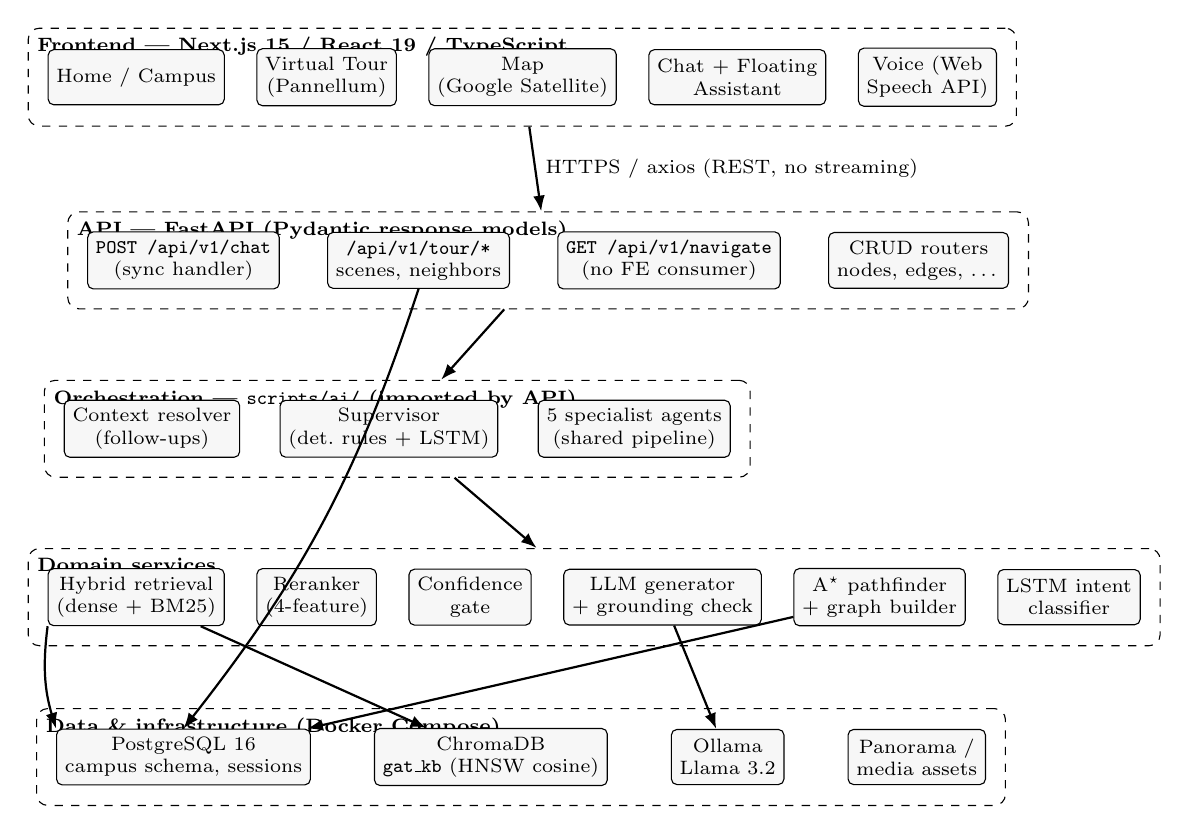
\begin{tikzpicture}[
  font=\scriptsize,
  box/.style={draw, rounded corners=2pt, align=center, minimum height=7mm, inner sep=3pt, fill=black!3},
  grp/.style={draw, dashed, rounded corners=4pt, inner sep=7pt},
  flow/.style={-{Latex[length=2mm]}, thick}
]
% ---- Frontend ----
\node[box] (home)  {Home / Campus};
\node[box, right=4mm of home] (tour) {Virtual Tour\\(Pannellum)};
\node[box, right=4mm of tour] (map) {Map\\(Google Satellite)};
\node[box, right=4mm of map] (chat) {Chat + Floating\\Assistant};
\node[box, right=4mm of chat] (voice) {Voice (Web\\Speech API)};
\begin{scope}[on background layer]
\node[grp, fit=(home)(tour)(map)(chat)(voice), label={[anchor=north west]north west:\textbf{Frontend --- Next.js 15 / React 19 / TypeScript}}] (fe) {};
\end{scope}

% ---- API layer ----
\node[box, below=16mm of home, xshift=6mm] (chatapi) {\code{POST /api/v1/chat}\\(sync handler)};
\node[box, right=6mm of chatapi] (tourapi) {\code{/api/v1/tour/*}\\scenes, neighbors};
\node[box, right=6mm of tourapi] (navapi) {\code{GET /api/v1/navigate}\\(no FE consumer)};
\node[box, right=6mm of navapi] (crud) {CRUD routers\\nodes, edges, \dots};
\begin{scope}[on background layer]
\node[grp, fit=(chatapi)(tourapi)(navapi)(crud), label={[anchor=north west]north west:\textbf{API --- FastAPI (Pydantic response models)}}] (api) {};
\end{scope}

% ---- Orchestration ----
\node[box, below=14mm of chatapi, xshift=-4mm] (ctx) {Context resolver\\(follow-ups)};
\node[box, right=5mm of ctx] (sup) {Supervisor\\(det.\ rules + LSTM)};
\node[box, right=5mm of sup] (agents) {5 specialist agents\\(shared pipeline)};
\begin{scope}[on background layer]
\node[grp, fit=(ctx)(sup)(agents), label={[anchor=north west]north west:\textbf{Orchestration --- \code{scripts/ai/} (imported by API)}}] (orch) {};
\end{scope}

% ---- Services ----
\node[box, below=14mm of ctx, xshift=-2mm] (retr) {Hybrid retrieval\\(dense + BM25)};
\node[box, right=4mm of retr] (rr) {Reranker\\(4-feature)};
\node[box, right=4mm of rr] (conf) {Confidence\\gate};
\node[box, right=4mm of conf] (gen) {LLM generator\\+ grounding check};
\node[box, right=4mm of gen] (nav) {A$^{\star}$ pathfinder\\+ graph builder};
\node[box, right=4mm of nav] (lstm) {LSTM intent\\classifier};
\begin{scope}[on background layer]
\node[grp, fit=(retr)(rr)(conf)(gen)(nav)(lstm), label={[anchor=north west]north west:\textbf{Domain services}}] (svc) {};
\end{scope}

% ---- Data / infra ----
\node[box, below=13mm of retr, xshift=6mm] (pg) {PostgreSQL 16\\campus schema, sessions};
\node[box, right=8mm of pg] (chroma) {ChromaDB\\\code{gat\_kb} (HNSW cosine)};
\node[box, right=8mm of chroma] (ollama) {Ollama\\Llama~3.2};
\node[box, right=8mm of ollama] (files) {Panorama /\\media assets};
\begin{scope}[on background layer]
\node[grp, fit=(pg)(chroma)(ollama)(files), label={[anchor=north west]north west:\textbf{Data \& infrastructure (Docker Compose)}}] (data) {};
\end{scope}

% edges
\draw[flow] (fe) -- node[right,font=\scriptsize]{HTTPS / axios (REST, no streaming)} (api);
\draw[flow] (api) -- (orch);
\draw[flow] (orch) -- (svc);
\draw[flow] (retr) -- (chroma);
\draw[flow] (retr.south west) to[bend right=12] (pg.north west);
\draw[flow] (gen) -- (ollama);
\draw[flow] (nav) -- (pg);
\draw[flow] (tourapi.south) to[bend left=10] (pg.north);
\end{tikzpicture}
\caption{\system{} system architecture, reconstructed from the implemented
import graph. The RAG/agent pipeline lives in \code{scripts/ai/} and is
imported into the FastAPI process via a \code{sys.path} insertion; the
navigation engine lives in \code{backend/app/navigation/}. The chat handler
is a synchronous route dispatched on Starlette's thread pool. There is
currently no front-end consumer of \code{/api/v1/navigate}.}
\label{fig:arch}
\end{figure*}

\begin{figure}[!t]
\centering
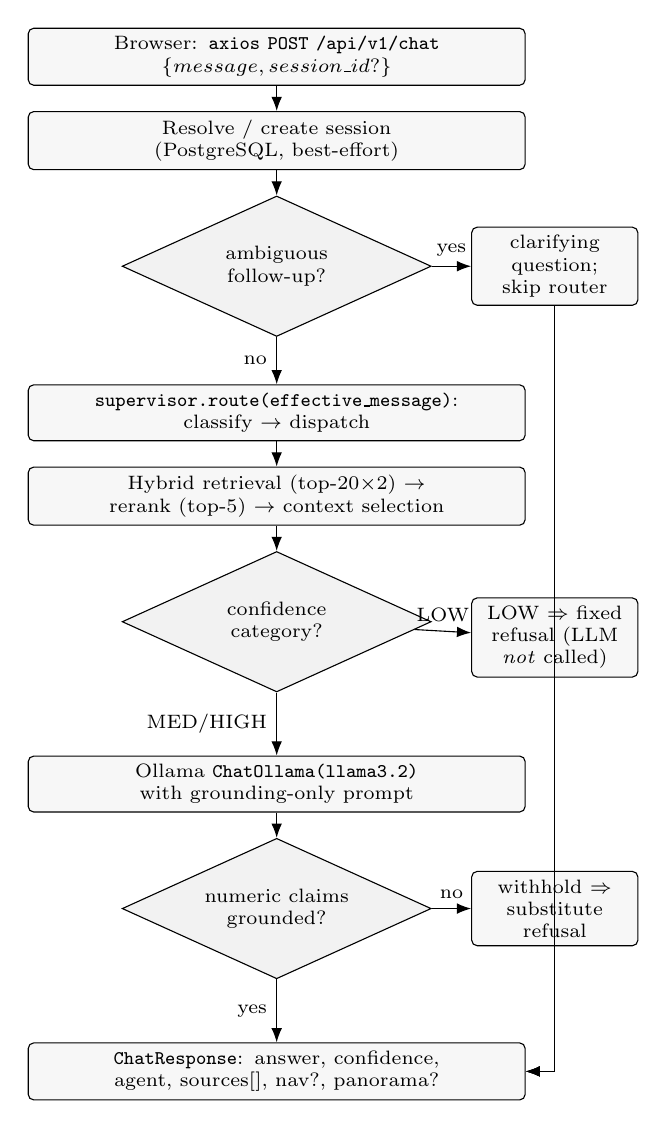
\begin{tikzpicture}[
  font=\scriptsize,
  node distance=3.2mm,
  b/.style={draw, rounded corners=2pt, align=center, text width=6.1cm, minimum height=6mm, inner sep=3pt, fill=black!3},
  d/.style={draw, diamond, aspect=2.2, align=center, inner sep=1pt, text width=2.6cm, fill=black!5},
  pf/.style={-{Latex[length=1.8mm]}}
]
\node[b] (inp) {Browser: \code{axios POST /api/v1/chat} $\{message, session\_id?\}$};
\node[b, below=of inp] (sess) {Resolve / create session (PostgreSQL, best-effort)};
\node[d, below=of sess] (amb) {ambiguous\\follow-up?};
\node[b, below=6mm of amb] (route) {\code{supervisor.route(effective\_message)}: classify $\rightarrow$ dispatch};
\node[b, below=of route] (retr) {Hybrid retrieval (top-20$\times$2) $\rightarrow$ rerank (top-5) $\rightarrow$ context selection};
\node[d, below=of retr] (cat) {confidence\\category?};
\node[b, below=8mm of cat] (llm) {Ollama \code{ChatOllama(llama3.2)} with grounding-only prompt};
\node[d, below=of llm] (grd) {numeric claims\\grounded?};
\node[b, below=8mm of grd] (out) {\code{ChatResponse}: answer, confidence, agent, sources[], nav?, panorama?};
\node[b, right=5mm of cat, text width=1.9cm, yshift=-2mm] (refuse) {LOW $\Rightarrow$ fixed refusal (LLM \emph{not} called)};
\node[b, right=5mm of grd, text width=1.9cm] (with) {withhold $\Rightarrow$ substitute refusal};
\node[b, right=5mm of amb, text width=1.9cm] (clar) {clarifying question; skip router};

\draw[pf] (inp)--(sess);
\draw[pf] (sess)--(amb);
\draw[pf] (amb)-- node[left]{no} (route);
\draw[pf] (amb)-- node[above]{yes} (clar);
\draw[pf] (route)--(retr);
\draw[pf] (retr)--(cat);
\draw[pf] (cat)-- node[left]{MED/HIGH} (llm);
\draw[pf] (cat)-- node[above]{LOW} (refuse);
\draw[pf] (llm)--(grd);
\draw[pf] (grd)-- node[left]{yes} (out);
\draw[pf] (grd)-- node[above]{no} (with);
\draw[pf] (clar) |- (out);
\draw[pf] (refuse) |- (out);
\draw[pf] (with) |- (out);
\end{tikzpicture}
\caption{End-to-end request flow for a chat query. The confidence gate and
the post-generation grounding check are two independent points at which the
system substitutes a fixed refusal for a generated answer.}
\label{fig:reqflow}
\end{figure}


\system{} is a four-tier web application (Fig.~\ref{fig:arch}): a
single-page front end, a versioned HTTP API, an orchestration layer, and a
set of domain services backed by relational, vector, model-serving, and
file infrastructure. The architecture was reconstructed for this paper
directly from the implemented import graph rather than from design
documents, several of which are stale relative to the code.

\subsection{Tier 1 --- Front End}
The front end is a Next.js~15 App-Router application in TypeScript
(\code{strict} mode). Routes are thin compositions of feature components;
all HTTP traffic is funnelled through a single \code{axios} client layer;
server state is held in TanStack Query caches and cross-component client
state in three Zustand stores (chat, campus, language). The five
user-facing surfaces are the landing/campus pages, the Pannellum-based
360$^{\circ}$ tour, a Google-satellite map view, a full-page chat, and a
site-wide floating assistant that mounts the same chat component in a
compact panel. Voice input is a browser-native Web Speech API hook that
writes its transcript into the ordinary chat send path.

\subsection{Tier 2 --- API}
The API is a FastAPI application. Every route declares a Pydantic
\code{response\_model}; cross-origin access is restricted to configured
origins. The chat route, \code{POST /api/v1/chat}, is deliberately a
\emph{synchronous} handler: the entire downstream pipeline (ChromaDB
queries, sentence-transformer encoding, SQLAlchemy calls, the Ollama HTTP
call) is blocking code, and Starlette dispatches synchronous handlers on a
thread pool, so a slow request does not block the event loop. Tour data is
served by \code{/api/v1/tour/*}; the campus graph is exposed through
generic CRUD routers; and \code{GET /api/v1/navigate} exposes the
A$^{\star}$ engine (it currently has no front-end consumer).

\subsection{Tier 3 --- Orchestration}
The RAG and multi-agent logic resides in \code{scripts/ai/} and is imported
into the FastAPI process by inserting that directory on \code{sys.path}.
This is a documented deviation from the repository's own folder convention,
made so that each pipeline stage remains independently runnable and
testable outside a live server. The chat handler performs three steps:
(i)~best-effort session resolution against PostgreSQL; (ii)~contextual
follow-up resolution, which may short-circuit the request with a clarifying
question when a pronominal reference is ambiguous; and (iii)~a single call
into \code{supervisor.route()}, which is the sole path from the HTTP layer
into the AI pipeline. Figure~\ref{fig:reqflow} shows the full flow.

\subsection{Tier 4 --- Domain Services and Infrastructure}
Six domain services are invoked by the orchestration layer: hybrid
retrieval, reranking, confidence estimation, grounded generation (with the
post-hoc grounding check), the A$^{\star}$ pathfinder with its graph
builder, and the LSTM intent classifier. Infrastructure comprises
PostgreSQL~16 (the campus schema and chat-session persistence), an
on-disk ChromaDB collection with an HNSW cosine index, an Ollama server
hosting Llama~3.2, and a panorama/media asset tree. Docker Compose defines
exactly four services (\code{frontend}, \code{backend}, \code{db},
\code{ollama}); there is no cache or queue service.

\subsection{Shared Campus Model}
All three subsystems key off one relational model:
$\textsf{Campus}\!\rightarrow\!\textsf{Building}\!\rightarrow\!\textsf{Floor}\!\rightarrow\!\textsf{Room}$,
with a central $\textsf{Node}$ table (the graph vertex) that a $\textsf{Room}$
optionally maps to one-to-one, $\textsf{Edge}$ rows forming the navigation
graph, and $\textsf{Panorama}$ rows attaching tour imagery to nodes. The
tour's scene list, the minimap's coordinates, and the pathfinder's graph
are three views of this same data; there is no separate graph file. This
shared model is what makes the integration (objective~O and constraint~P5)
concrete rather than nominal: a node added for wayfinding is immediately a
candidate tour scene and a minimap point.

\subsection{Key Data Contracts}
The chat contract is
$\{message,\ session\_id?,\ language?\}\rightarrow\{answer,\ status,\
confidence,\ confidence\_level,\ selected\_agent,\ tool\_used,\
sources[],\ navigation?,\ panorama?,\ session\_id\}$.
The navigation contract is
$\{start\_node\_id,\ destination\_node\_id,\ accessible\_only\}\rightarrow
\{path\_node\_ids,\ path\_node\_names,\ total\_distance,\
estimated\_walk\_time\_minutes,\ is\_accessible,\ turn\_by\_turn[]\}$.
Every AI-generated answer carries its grounding sources as a structural
field, and those sources are always built from retrieved-chunk metadata,
never parsed from the model's text.

\section{Campus Knowledge Representation and Dataset}
\label{sec:dataset}
\begin{figure}[!t]
\centering
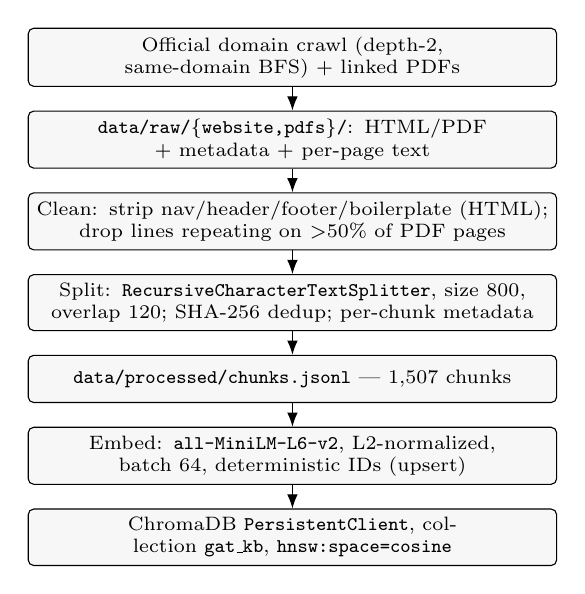
\begin{tikzpicture}[
  font=\scriptsize, node distance=3mm,
  b/.style={draw, rounded corners=2pt, align=center, text width=6.5cm, minimum height=6mm, inner sep=3pt, fill=black!3},
  pf/.style={-{Latex[length=1.8mm]}}
]
\node[b] (src) {Official domain crawl (depth-2, same-domain BFS) + linked PDFs};
\node[b, below=of src] (raw) {\code{data/raw/\{website,pdfs\}/}: HTML/PDF + metadata + per-page text};
\node[b, below=of raw] (clean) {Clean: strip nav/header/footer/boilerplate (HTML); drop lines repeating on $>$50\% of PDF pages};
\node[b, below=of clean] (chunk) {Split: \code{RecursiveCharacterTextSplitter}, size 800, overlap 120; SHA-256 dedup; per-chunk metadata};
\node[b, below=of chunk] (jsonl) {\code{data/processed/chunks.jsonl} --- 1{,}507 chunks};
\node[b, below=of jsonl] (emb) {Embed: \code{all-MiniLM-L6-v2}, L2-normalized, batch 64, deterministic IDs (upsert)};
\node[b, below=of emb] (store) {ChromaDB \code{PersistentClient}, collection \code{gat\_kb}, \code{hnsw:space=cosine}};
\draw[pf] (src)--(raw); \draw[pf] (raw)--(clean); \draw[pf] (clean)--(chunk);
\draw[pf] (chunk)--(jsonl); \draw[pf] (jsonl)--(emb); \draw[pf] (emb)--(store);
\end{tikzpicture}
\caption{Offline knowledge-base construction pipeline
(\code{scripts/ai/}). Every stage is independently runnable; the source
manifest records each URL's status (collected / chunked / embedded /
failed-with-reason).}
\label{fig:kbpipe}
\end{figure}

\begin{figure}[!t]
\centering
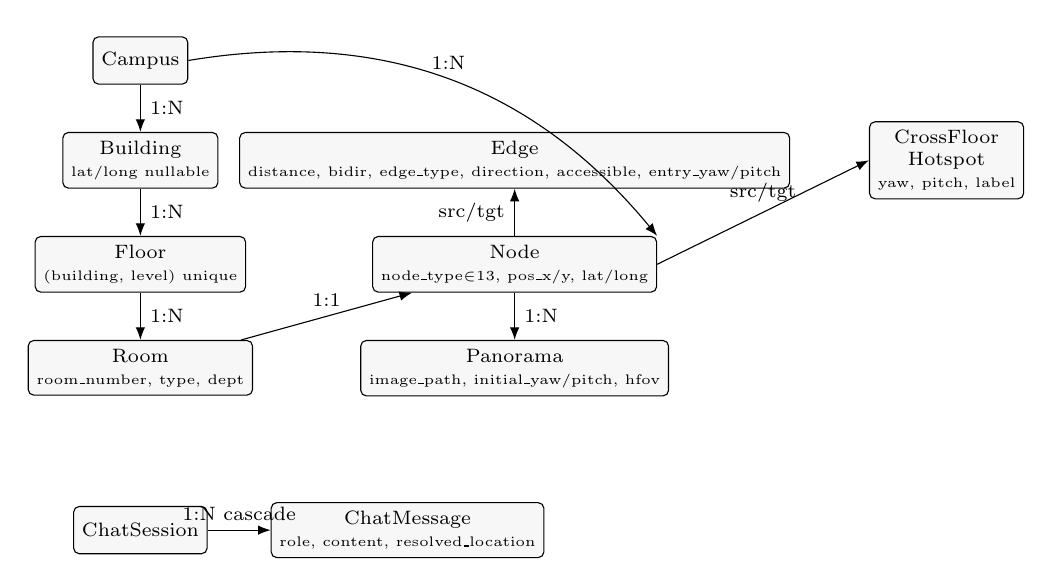
\begin{tikzpicture}[
  font=\scriptsize, node distance=6mm and 8mm,
  e/.style={draw, rounded corners=2pt, align=center, minimum height=6mm, inner sep=3pt, fill=black!3},
  rel/.style={draw, -{Latex[length=1.6mm]}}
]
\node[e] (campus) {Campus};
\node[e, below=of campus] (building) {Building\\{\tiny lat/long nullable}};
\node[e, below=of building] (floor) {Floor\\{\tiny (building, level) unique}};
\node[e, below=of floor] (room) {Room\\{\tiny room\_number, type, dept}};
\node[e, right=16mm of floor] (nd) {Node\\{\tiny node\_type$\in$13, pos\_x/y, lat/long}};
\node[e, above=of nd] (eg) {Edge\\{\tiny distance, bidir, edge\_type, direction, accessible, entry\_yaw/pitch}};
\node[e, below=of nd] (pano) {Panorama\\{\tiny image\_path, initial\_yaw/pitch, hfov}};
\node[e, right=10mm of eg] (cfh) {CrossFloor\\Hotspot\\{\tiny yaw, pitch, label}};
\node[e, below=14mm of room] (sess) {ChatSession};
\node[e, right=8mm of sess] (msg) {ChatMessage\\{\tiny role, content, resolved\_location}};

\draw[rel] (campus) -- node[right]{1:N} (building);
\draw[rel] (building) -- node[right]{1:N} (floor);
\draw[rel] (floor) -- node[right]{1:N} (room);
\draw[rel] (room) -- node[above]{1:1} (nd);
\draw[rel] (nd) -- node[right]{1:N} (pano);
\draw[rel] (nd.north) -- node[left]{src/tgt} (eg.south);
\draw[rel] (nd.east) -- node[above]{src/tgt} (cfh.west);
\draw[rel] (campus.east) to[bend left=30] node[above]{1:N} (nd.north east);
\draw[rel] (sess) -- node[above]{1:N cascade} (msg);
\end{tikzpicture}
\caption{Campus relational model (SQLAlchemy). The \textsf{Node} table is
the single graph vertex used by pathfinding, tour scenes, and the minimap;
\textsf{CrossFloorHotspot} is a visual sightline layer and is \emph{not}
part of the pathfinding graph.}
\label{fig:er}
\end{figure}

\begin{table}[!t]
\centering
\caption{Verified Implementation-Scale Measurements. These are
\emph{dataset/implementation} metrics, not performance results.}
\label{tab:counts}
\footnotesize
\renewcommand{\arraystretch}{1.15}
\begin{tabular}{@{}p{5.4cm}r@{}}
\toprule
\textbf{Asset / quantity} & \textbf{Value} \\
\midrule
Knowledge-base text chunks (\code{chunks.jsonl}, embedded) & 1{,}507 \\
Source PDFs on disk & 128 \\
Source website pages on disk & 42 \\
Cumulative unique source URLs ever attempted & 186 \\
\quad PDFs chunked / failed & 70 / 71 \\
\quad Website pages chunked / failed & 40 / 5 \\
Chunk size / overlap (characters) & 800 / 120 \\
Embedding model / dimension & MiniLM-L6 / 384 \\
\midrule
Campus graph nodes & 180 \\
Campus graph edges & 325 \\
Panorama scenes (database rows) & 161 \\
Panorama image files (main building tree) & $\approx$178 \\
Floors / buildings / campuses & 10 / 5 / 1 \\
Rooms (relational) & 11 \\
Cross-floor hotspots & 849 \\
\midrule
Accumulated chat sessions (development) & 378 \\
Accumulated chat messages (development) & 1{,}400 \\
\midrule
Intent classifier: training / validation examples & 134 / 34 \\
Intent classifier: classes & 12 \\
Intent classifier: vocabulary size & 283 \\
Alembic migration revisions & 14 \\
\bottomrule
\end{tabular}
\end{table}


\system{} maintains two deliberately separate knowledge stores: an
\emph{institutional} store (unstructured text in ChromaDB, for the RAG
assistant) and a \emph{spatial} store (the relational campus model in
PostgreSQL, for the tour and the pathfinder). They are never merged; a
chunk is tagged \code{knowledge\_category = "official\_institutional"} and
spatial facts are never scraped or inferred into it.

\subsection{Institutional Knowledge Base}
The knowledge base is built offline by the pipeline of
Fig.~\ref{fig:kbpipe} and Algorithm~\ref{alg:kb}. A polite depth-2
same-domain breadth-first crawl of the institution's website records every
page and every linked PDF; a separate collector downloads the PDFs and
extracts per-page text. Cleaning removes navigation, header, footer, and
cookie-banner boilerplate from HTML (by tag and by class/id hint) and
removes running headers/footers from PDFs by dropping any line that appears
on more than half of a document's pages. Text is split with a recursive
character splitter (chunk size $800$, overlap $120$, separator preference
\code{["\textbackslash n\textbackslash n", "\textbackslash n", ". ", " "]}).
Each chunk is fingerprinted by the SHA-256 hash of its whitespace-collapsed,
lower-cased text, and the first occurrence of any duplicate wins. Every
surviving chunk carries \code{chunk\_id}, \code{source\_url},
\code{source\_title}, \code{source\_type}, \code{section} (nearest preceding
heading, for web pages), \code{page} (exact, for PDFs), \code{document\_name},
a best-effort \code{department} label from URL pattern matching, and a
collection date.

The current build contains $1{,}507$ chunks. The cumulative source manifest
records $186$ unique URLs ever attempted, with typed failure reasons (most
commonly ``no extractable text --- likely scanned/image-only PDF''); nothing
is silently dropped. Chunks are embedded with \code{all-MiniLM-L6-v2}
(384-dimensional, L2-normalized)~\cite{sbertlib} in batches of $64$ and
upserted into the persistent ChromaDB collection~\cite{chroma2023}
\code{gat\_kb} with \code{hnsw:space = cosine}. Chunk identifiers are deterministic, so re-running the pipeline
updates rather than duplicates records. A direct query against the
persisted store confirms the collection holds exactly $1{,}507$ records,
i.e.\ the pipeline has been executed end to end.

\begin{algorithm}[!t]
\caption{Institutional Knowledge Acquisition and Chunking}
\label{alg:kb}
\begin{algorithmic}[1]
\Require seed URL $u_0$; domain $\delta$; sizes $c=800$, $o=120$
\Ensure chunk records $\mathcal{C}$; embedded collection \code{gat\_kb}
\State $\mathcal{R}\gets \textsc{Crawl}(u_0,\delta,\text{depth}{=}2)$;
       $\mathcal{F}\gets$ PDF links found in $\mathcal{R}$
\State download and per-page-extract each $f\in\mathcal{F}$ ($\le 15$\,MB)
\State $\mathcal{C}\gets\emptyset$;\ \ $H\gets\emptyset$ \Comment{seen SHA-256 fingerprints}
\ForAll{documents $d \in \mathcal{R}\cup\mathcal{F}$}
  \If{$d$ is HTML}
     \State $t\gets\textsc{StripBoilerplate}(d)$; track nearest heading per span
  \Else
     \State $P\gets$ pages of $d$;\ drop lines on $>\!\tfrac{|P|}{2}$ pages;\ $t\gets P$
  \EndIf
  \State $K\gets \textsc{RecursiveSplit}(t, c, o)$
  \ForAll{$k \in K$}
     \State $h\gets \textsc{SHA256}(\textsc{Normalize}(k))$
     \If{$h \notin H$}
        \State $H\gets H\cup\{h\}$
        \State attach $\{$\code{source\_url}, \code{section}, \code{page},
               \code{department}, $\dots\}$ to $k$
        \State $\mathcal{C}\gets\mathcal{C}\cup\{k\}$
     \EndIf
  \EndFor
\EndFor
\ForAll{batches $B$ of $\mathcal{C}$ ($|B|\le 64$)}
  \State $\bm{e}\gets \textsc{Encode}_{\text{MiniLM}}(B)$;\ normalize $\|\bm{e}\|_2{=}1$
  \State \code{gat\_kb.upsert}(ids$(B)$, $\bm{e}$, text$(B)$, meta$(B)$)
\EndFor
\end{algorithmic}
\end{algorithm}

\subsection{Spatial / Relational Campus Model}
The relational model (Fig.~\ref{fig:er}) is the single source of truth for
everything spatial. A $\textsf{Node}$ has a $13$-value type enumeration
(entrance, junction, corridor, room, staircase, elevator, landmark,
outdoor, classroom, lab, office, library, cafeteria), optional planar
coordinates $(\text{pos\_x}, \text{pos\_y})$, and optional geographic
coordinates. An $\textsf{Edge}$ is directed with a \code{distance}, an
\code{is\_bidirectional} flag, a $6$-value \code{edge\_type}, a $6$-value
relative \code{direction} (for turn-by-turn phrasing), an \code{accessible}
flag, and optional \code{entry\_yaw}/\code{entry\_pitch} for tour-hotspot
placement. A $\textsf{Panorama}$ attaches to a node and carries a resting
\code{initial\_yaw}/\code{initial\_pitch} and horizontal field of view.
$\textsf{CrossFloorHotspot}$ rows are a hand-authored visual sightline
layer and are explicitly excluded from the pathfinding graph.

The live database contains $180$ nodes, $325$ edges, $161$ panorama rows,
$849$ cross-floor hotspots, $10$ floors, $5$ buildings, and $11$ relational
rooms (Table~\ref{tab:counts}). Fourteen Alembic migrations define the
schema history, including one feature (visibility zones) that was added and
later reverted. All building \code{latitude}/\code{longitude} values are
currently null; the only geographic coordinate in the system is a single
campus-level point sourced from public third-party map data and documented
as unsurveyed. Panorama imagery and coordinates are placeholders by design;
the code path from placeholder to real assets is a file/identifier
substitution.

\subsection{Development Usage Evidence}
The chat-session tables have accumulated $378$ sessions and $1{,}400$
messages during development. This is not an experimental result --- it is
evidence that the end-to-end path (front end $\to$ API $\to$ supervisor
$\to$ retrieval $\to$ Ollama $\to$ persistence) has been exercised against
a live stack rather than only unit-tested.

\section{Virtual Campus and 360$^{\circ}$ Tour Engine}
\label{sec:tour}
\begin{figure}[!t]
\centering
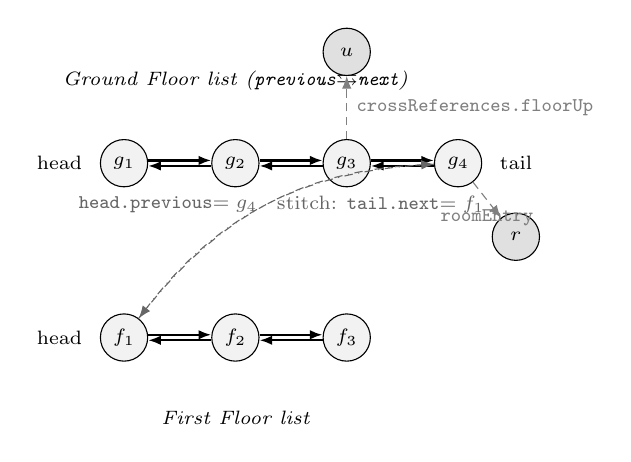
\begin{tikzpicture}[
  font=\scriptsize, node distance=8mm,
  n/.style={draw, circle, minimum size=6mm, inner sep=0pt, fill=black!5},
  chain/.style={-{Latex[length=1.6mm]}, thick},
  xref/.style={-{Latex[length=1.6mm]}, densely dashed, gray},
  cf/.style={-{Latex[length=1.6mm]}, dash dot, black!60}
]
% ground floor chain
\node[n] (g1) {$g_1$};
\node[n, right=of g1] (g2) {$g_2$};
\node[n, right=of g2] (g3) {$g_3$};
\node[n, right=of g3] (g4) {$g_4$};
\node[left=1mm of g1] {head};
\node[right=1mm of g4] {tail};
\draw[chain, transform canvas={yshift=1pt}] (g1)--(g2);
\draw[chain, transform canvas={yshift=-1pt}] (g2)--(g1);
\draw[chain, transform canvas={yshift=1pt}] (g2)--(g3);
\draw[chain, transform canvas={yshift=-1pt}] (g3)--(g2);
\draw[chain, transform canvas={yshift=1pt}] (g3)--(g4);
\draw[chain, transform canvas={yshift=-1pt}] (g4)--(g3);
\node[above=5mm of g2, font=\scriptsize\itshape] {Ground Floor list (\code{previous}$\leftrightarrows$\code{next})};

% first floor chain
\node[n, below=16mm of g1] (f1) {$f_1$};
\node[n, right=of f1] (f2) {$f_2$};
\node[n, right=of f2] (f3) {$f_3$};
\node[left=1mm of f1] {head};
\draw[chain, transform canvas={yshift=1pt}] (f1)--(f2);
\draw[chain, transform canvas={yshift=-1pt}] (f2)--(f1);
\draw[chain, transform canvas={yshift=1pt}] (f2)--(f3);
\draw[chain, transform canvas={yshift=-1pt}] (f3)--(f2);
\node[below=5mm of f2, font=\scriptsize\itshape] {First Floor list};

% cross-floor stitch tail(g)->head(f)
\draw[cf, bend right=25] (g4) to node[right, font=\scriptsize] {stitch: \code{tail.next}$=f_1$} (f1);
\draw[cf, bend left=25] (f1) to node[left, font=\scriptsize] {\code{head.previous}$=g_4$} (g4);

% cross references
\node[n, above=8mm of g3, fill=black!12] (up) {$u$};
\draw[xref] (g3) to node[right, font=\scriptsize] {\code{crossReferences.floorUp}} (up);
\node[n, below right=5mm and 3mm of g4, fill=black!12] (room) {$r$};
\draw[xref] (g4) to node[below, font=\scriptsize] {\code{roomEntry}} (room);
\end{tikzpicture}
\caption{Panorama scene graph. Each floor is a doubly linked list (solid);
branch and vertical connections are separate cross-reference pointers
(dashed); a construction pass stitches each floor's tail to the next
floor's head (dash-dot), so sequential traversal crosses floors with no
boundary-aware code.}
\label{fig:scenegraph}
\end{figure}

\begin{figure}[!t]
\centering
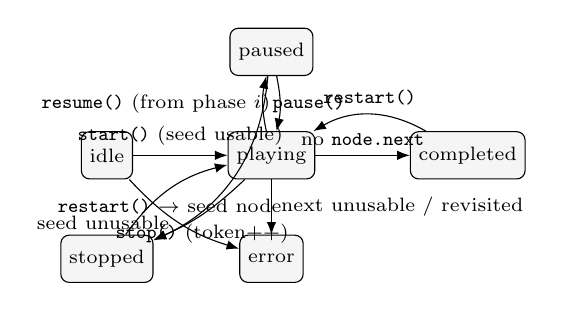
\begin{tikzpicture}[
  font=\scriptsize, node distance=7mm and 12mm,
  s/.style={draw, rounded corners=3pt, minimum height=6mm, inner sep=3pt, fill=black!4},
  pf/.style={-{Latex[length=1.6mm]}}
]
\node[s] (idle) {idle};
\node[s, right=of idle] (play) {playing};
\node[s, above=of play] (pause) {paused};
\node[s, right=of play] (done) {completed};
\node[s, below=of play] (err) {error};
\node[s, below=of idle] (stop) {stopped};

\draw[pf] (idle) -- node[above]{\code{start()} (seed usable)} (play);
\draw[pf] (idle) to[bend right=15] node[left]{seed unusable} (err);
\draw[pf] (play) to[bend left=12] node[right]{\code{pause()}} (pause);
\draw[pf] (pause) to[bend left=12] node[left]{\code{resume()} (from phase $i$)} (play);
\draw[pf] (play) -- node[above]{no \code{node.next}} (done);
\draw[pf] (play) -- node[right]{next unusable / revisited} (err);
\draw[pf] (play) to[bend left=10] node[below]{\code{stop()} (token${+}{+}$)} (stop);
\draw[pf] (pause) to[bend left=30] (stop);
\draw[pf] (stop) to[bend left=20] node[below]{\code{restart()} $\to$ seed node} (play);
\draw[pf] (done) to[bend right=30] node[above]{\code{restart()}} (play);
\end{tikzpicture}
\caption{Guided-tour status automaton (\code{useGuidedTour}). A monotonic
cancellation token orphans in-flight timer chains on every transition out
of \emph{playing}; a per-run visited set aborts to \emph{error} on a
repeated scene.}
\label{fig:guided}
\end{figure}


The tour is not merely a set of 360$^{\circ}$ images: it is a data
structure over which two traversal modes operate. This section describes
the scene graph, the cross-floor stitching pass, the manual and guided
traversal algorithms, and the minimap projection, all as implemented in
\code{frontend/src/features/tour/engine/}.

\subsection{Scene-Graph Data Structure}
The overall structure is shown in Fig.~\ref{fig:scenegraph}. Each panorama
scene is a \code{PanoramaNode} object holding an image path,
a preview path, a resting orientation $(\mathrm{yaw}, \mathrm{pitch},
\mathrm{hfov})$, a $1$-based per-floor sequence index, \code{previous} and
\code{next} links, a \code{crossReferences} record, and a list of
hand-authored \code{crossFloorHotspots}. A link
$\ell = (\text{node}, \mathrm{entryYaw}, \mathrm{entryPitch})$ carries the
camera heading the target should open with when reached \emph{via that
link}, in the Street-View style~\cite{anguelov2010streetview} of preserving
the direction of travel.

Each floor is a \code{PanoramaLinkedList}: a doubly linked list with
\code{head}/\code{tail} pointers and a \code{Map}$\langle$id$,$node$\rangle$
for $O(1)$ random access. Sequential traversal is $O(1)$ per step; the
list's \code{toArray()} deliberately stops at its own \code{tail} rather
than following \code{next} indefinitely, because after stitching a tail's
\code{next} points into another floor. The whole building is a
\code{PanoramaEngine}: a \code{Map}$\langle$floorName$,$list$\rangle$ plus a
flat node index, built once per tour-page render by \code{useMemo} directly
from the backend \code{/tour/scenes} response --- never a hardcoded array.

\emph{Why a doubly linked list.} A flat array with \code{findIndex} (the
prior design) makes ``next scene'' an $O(n)$ scan and couples every
consumer to array positions; a modulo wraparound over the array also
produces an artificial jump from the last scene back to the first. A
general graph structure would support the branch connections but makes
``the next scene in the walking sequence'' ill-defined. The doubly linked
list gives $O(1)$ ordered traversal, a natural place to attach
per-direction entry orientation, and a per-floor \code{size} for the
``scene $x$ of $y$'' indicator; branch and vertical connections that are
\emph{not} part of the walking sequence are held separately in
\code{crossReferences} (opposite corridor, floor up/down, lift array, room
entry, return-to-corridor). This separation is the core data-structure
decision.

\subsection{Engine Construction}
\code{buildPanoramaEngine} runs four passes. \emph{Pass~1} groups scenes by
floor, sorts each group by stored sequence index, and appends nodes to that
floor's list; forward entry orientation is the target's own calibrated
$(\mathrm{yaw},\mathrm{pitch})$ and backward entry orientation is the
source's yaw $+180^{\circ}$ --- both read live from calibration, never from
a stored (possibly stale) edge value. \emph{Pass~2} converts each scene's
non-chain hotspots into \code{crossReferences} pointers (an
\code{elevator} hotspot appends to the \code{lift} array; \code{upstairs}
sets \code{floorUp}; etc.). \emph{Pass~3} is cross-floor stitching
(Algorithm~\ref{alg:crossfloor}). \emph{Pass~4} attaches each
hand-authored cross-floor sightline hotspot to exactly the node it was
authored on, skipping rows whose source node cannot be resolved.

A read-time reclassification moves the ground floor's calibrated scene~$5$
--- a standalone courtyard view --- into its own single-scene floor bucket
``Central Quadrangle,'' closing the gap in the ground-floor sequence around
it. The underlying scene object is untouched; only its floor grouping
changes. This is why the tour's floor sequence has six entries over five
physical floor directories.

\subsection{Cross-Floor Stitching}
\begin{algorithm}[!t]
\caption{Cross-Floor Panorama Stitching (Pass 3)}
\label{alg:crossfloor}
\begin{algorithmic}[1]
\Require engine $\mathcal{E}$; ordered floor sequence
$\Phi = \langle\text{Entrance},\text{Ground},\text{First},\text{Second},\text{Third},\text{Quadrangle}\rangle$
\Ensure each floor's tail linked to the next floor's head
\For{$i \gets 1$ \textbf{to} $|\Phi|-1$}
  \State $L \gets \mathcal{E}.\text{getFloor}(\Phi_i)$;\ \ $U \gets \mathcal{E}.\text{getFloor}(\Phi_{i+1})$
  \If{$L{.}\text{tail} = \varnothing \ \lor\ U{.}\text{head} = \varnothing$} \textbf{continue} \EndIf
  \State $a \gets L{.}\text{tail}$;\ \ $b \gets U{.}\text{head}$
  \State $a{.}\text{next} \gets (\,b,\ \mathrm{entryYaw}{=}b{.}\text{yaw},\ \mathrm{entryPitch}{=}b{.}\text{pitch}\,)$
  \State $b{.}\text{previous} \gets (\,a,\ \mathrm{entryYaw}{=}a{.}\text{yaw}{+}180^{\circ},\ \mathrm{entryPitch}{=}a{.}\text{pitch}\,)$
\EndFor
\end{algorithmic}
\end{algorithm}

Algorithm~\ref{alg:crossfloor} runs \emph{after} all six per-floor lists
exist. It wires a lower floor's tail to an upper floor's head using exactly
the same link shape and the same entry-orientation rule as an ordinary
same-floor link. Because manual \code{goToOffset($\pm1$)} and guided
auto-advance both read only \code{node.next}/\code{node.previous}, a scene
at the end of its floor transparently continues into the next floor's first
scene, \emph{with no code path aware that a boundary was crossed}. Each
floor's own list (\code{head}/\code{tail}/\code{size}) is untouched, so
``scene $x$ of $y$'' still counts within a floor. By design there is no
wraparound from the last floor back to the first.

\subsection{Manual Traversal}
\begin{algorithm}[!t]
\caption{Manual Tour Hotspot Derivation and Step}
\label{alg:tourwalk}
\begin{algorithmic}[1]
\Require current node $v$; requested offset $\Delta\in\{-1,+1\}$ or hotspot $k$
\Ensure next scene id and entry orientation
\State $H \gets \emptyset$ \Comment{navigable hotspots, derived, never stored}
\If{$v{.}\text{next} \ne \varnothing$}\ $H \mathrel{+}= (\text{forward},\ v{.}\text{next})$ at yaw $v{.}\text{yaw}$ \EndIf
\If{$v{.}\text{previous} \ne \varnothing$}\ $H \mathrel{+}= (\text{back},\ v{.}\text{previous})$ at yaw $v{.}\text{yaw}{+}180^{\circ}$ \EndIf
\ForAll{$c \in \{$oppositeCorridor, floorUp, floorDown, lift$[\,]$, roomEntry, returnTo$\}$}
  \If{$v{.}\text{crossReferences}[c] \ne \varnothing$ \textbf{and} a raw edge angle exists}
     \State $H \mathrel{+}= (c,\ \text{target})$ at that edge's $(\mathrm{yaw},\mathrm{pitch})$
  \EndIf
\EndFor
\ForAll{$s \in v{.}\text{crossFloorHotspots}$}\ $H \mathrel{+}= (\text{crossFloor},\ s.\text{target})$ at $(s.\text{yaw},s.\text{pitch})$ \EndFor
\If{step is $\Delta$}
  \State $\ell \gets (\Delta = +1)\ ?\ v{.}\text{next} : v{.}\text{previous}$;\ \textbf{return} $(\ell{.}\text{node.id},\ \ell{.}\text{entryYaw},\ \ell{.}\text{entryPitch})$
\Else
  \State \textbf{return} target of hotspot $k$ with its authored entry orientation
\EndIf
\end{algorithmic}
\end{algorithm}
Every navigable hotspot is derived from the node's own links and
cross-references on each render (Algorithm~\ref{alg:tourwalk}); there is no
stored hotspot array and no manual enable/disable switch. Forward/back
hotspots are placed at the node's calibrated yaw and yaw~$+180^{\circ}$;
junction hotspots use the real edge angle because a corridor branch has no
fixed offset from ``forward.'' A lift with more than one reachable floor
renders a floor-select submenu.

\subsection{Guided Tour}
The guided tour is an automatic node-to-node walk driven entirely by
\code{node.next} object references (Fig.~\ref{fig:guided},
Algorithm~\ref{alg:guided}). At each node a fixed six-phase sequence runs:
\emph{pause} ($900$\,ms) $\to$ \emph{look-left} ($900$\,ms, $-40^{\circ}$)
$\to$ \emph{recenter} ($800$\,ms) $\to$ \emph{look-right} ($900$\,ms,
$+40^{\circ}$) $\to$ \emph{recenter} ($800$\,ms) $\to$ \emph{move}
($400$\,ms), with all durations scaled by a speed factor
($\times1.6$ slow, $\times1$ normal, $\times0.55$ fast). Correctness relies
on two mechanisms: a monotonically increasing \emph{cancellation token}
that is incremented on every \code{stop}/\code{restart}/unmount so that any
in-flight timer continuation observes a token mismatch and returns; and a
per-run \emph{visited set} that aborts the walk to an \emph{error} state if
\code{node.next} ever points to an already-visited scene (a corrupt-graph
guard). Pause freezes at a phase boundary after the in-flight camera
animation completes; resume continues from exactly that phase index;
restart rewinds to the node the tour was seeded on. Advancing uses the same
\code{goToScene} path as a manual hotspot click, so the fade transition is
identical between modes.

\begin{algorithm}[!t]
\caption{Guided Tour Execution at a Node}
\label{alg:guided}
\begin{algorithmic}[1]
\Require node $v$; start phase index $j$; run token $\tau$
\Ensure camera walk; advance or terminate
\For{$i \gets j$ \textbf{to} $5$}
  \If{$\tau \ne \tau_{\text{current}}$}\ \textbf{return} \Comment{stopped/restarted} \EndIf
  \If{status $=$ \emph{paused}}\ save $i$;\ \textbf{return} \EndIf
  \State render phase $\phi_i$;\ \textbf{await} camera animation for
         $\lceil \text{base}(\phi_i)\cdot \text{scale(speed)}\rceil$ ms
\EndFor
\State $w \gets v{.}\text{next.node}$
\If{$w = \varnothing$}\ status $\gets$ \emph{completed};\ \textbf{return} \EndIf
\If{$\neg\textsc{Usable}(w)$ \textbf{or} $w{.}\text{id} \in \text{visited}$}\ status $\gets$ \emph{error};\ \textbf{return} \EndIf
\State visited $\gets$ visited $\cup\ \{w{.}\text{id}\}$
\State \textsc{Advance}$(w{.}\text{id},\ v{.}\text{next.entryYaw},\ v{.}\text{next.entryPitch})$
\State \textbf{recurse} with $(w, 0, \tau)$
\end{algorithmic}
\end{algorithm}

\subsection{Minimap Projection}
The minimap (Algorithm~\ref{alg:minimap}) is inline SVG. For the current
floor it collects scenes whose backing node has real
$(\text{pos\_x},\text{pos\_y})$ coordinates; if at least two exist it
fits their bounding box into an on-card plot region with an
aspect-preserving scale and draws the real edges between them. If fewer
than two positioned scenes exist it falls back to an evenly spaced strip
inside the same region --- it \emph{never invents a coordinate}. A live
heading needle reads the panorama viewer's yaw once per animation frame and
is rotated by direct DOM mutation, bypassing React state to avoid 60\,Hz
re-renders. The outer ``entrance zone / building zone'' frame is explicitly
decorative and not survey-derived.

\begin{algorithm}[!t]
\caption{Minimap Coordinate Projection}
\label{alg:minimap}
\begin{algorithmic}[1]
\Require current floor scenes $F$; node positions $\text{pos}[\cdot]$; plot rect $Z=(x,y,w,h)$; pad $p$
\Ensure screen points for markers and edges
\State $S \gets \{(s,\text{pos}[s]) : s\in F,\ \text{pos}[s]\ \text{defined}\}$
\If{$|S| \ge 2$}
  \State $(x_{\min},x_{\max},y_{\min},y_{\max}) \gets$ bounding box of $S$
  \State $\sigma \gets \min\!\big(\tfrac{w-2p}{\max(x_{\max}-x_{\min},1)},\ \tfrac{h-2p}{\max(y_{\max}-y_{\min},1)}\big)$
  \State center the scaled box in $Z$; \textbf{for each} $(s,(a,b))$:
         $c_x \gets o_x + (a-x_{\min})\sigma$, $c_y \gets o_y + (b-y_{\min})\sigma$
  \State draw edge $(u,v)$ iff both endpoints are in $S$
\Else
  \State place $|F|$ markers evenly on the horizontal midline of $Z$ \Comment{no coordinate invented}
\EndIf
\end{algorithmic}
\end{algorithm}

\section{Intelligent RAG-Based Campus Assistant}
\label{sec:rag}
\begin{figure}[!t]
\centering
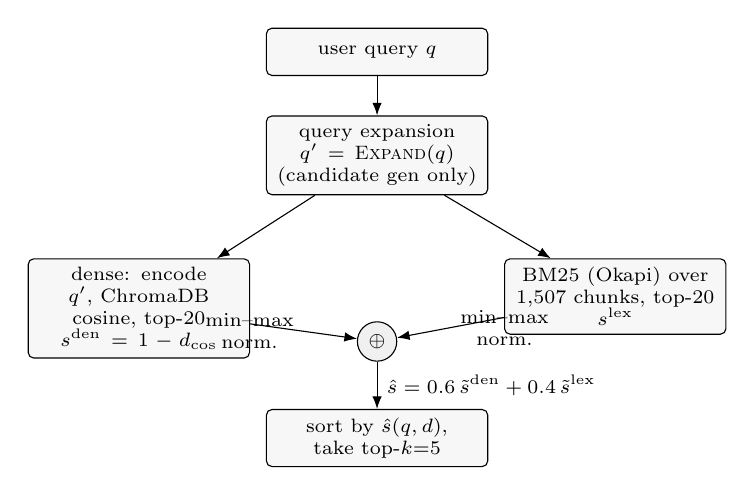
\begin{tikzpicture}[
  font=\scriptsize, node distance=5mm and 7mm,
  b/.style={draw, rounded corners=2pt, align=center, minimum height=6mm, inner sep=3pt, fill=black!3, text width=2.6cm},
  op/.style={draw, circle, inner sep=1pt, minimum size=5mm, fill=black!6},
  pf/.style={-{Latex[length=1.6mm]}}
]
\node[b] (q) {user query $q$};
\node[b, below=of q] (exp) {query expansion $q'=\textsc{Expand}(q)$ (candidate gen only)};
\node[b, below left=8mm and 2mm of exp] (dense) {dense: encode $q'$, ChromaDB cosine, top-20 \\ $s^{\text{den}}=1-d_{\cos}$};
\node[b, below right=8mm and 2mm of exp] (bm25) {BM25 (Okapi) over 1{,}507 chunks, top-20 \\ $s^{\text{lex}}$};
\node[op, below=16mm of exp] (fuse) {$\oplus$};
\node[b, below=6mm of fuse] (rank) {sort by $\hat s(q,d)$, take top-$k{=}5$};
\draw[pf] (q)--(exp);
\draw[pf] (exp)--(dense);
\draw[pf] (exp)--(bm25);
\draw[pf] (dense) -- node[left, align=center]{min--max\\norm.} (fuse);
\draw[pf] (bm25) -- node[right, align=center]{min--max\\norm.} (fuse);
\draw[pf] (fuse) -- node[right]{$\hat s = 0.6\,\tilde s^{\text{den}} + 0.4\,\tilde s^{\text{lex}}$} (rank);
\end{tikzpicture}
\caption{Hybrid retrieval. Query expansion widens only the candidate pool;
all downstream stages see the user's unmodified query. Each method's own
top-20 candidate scores are min--max normalized before the convex
combination.}
\label{fig:hybrid}
\end{figure}

\begin{table}[!t]
\centering
\caption{Qualitative Comparison of Retrieval Signals (No In-Domain
Effectiveness Measurement Has Been Performed; See Section~\ref{sec:eval}).}
\label{tab:retrieval}
\footnotesize
\renewcommand{\arraystretch}{1.2}
\begin{tabular}{@{}p{1.9cm}p{1.75cm}p{1.75cm}p{1.9cm}@{}}
\toprule
\textbf{Property} & \textbf{BM25 (lexical)} & \textbf{Dense (MiniLM)} & \textbf{Hybrid $0.6/0.4$ (implemented)} \\
\midrule
Paraphrase / synonymy & weak & strong & strong \\
Exact acronym / code / room \# & strong & weak--moderate & strong \\
Rare-term precision & strong & moderate & strong \\
Vocabulary-mismatch recall & weak & strong & strong \\
Keyword-coincidence noise & high & low & low (dense anchors) \\
Training data required & none & none (pretrained) & none \\
Index cost & low & moderate (HNSW) & sum of both \\
Query latency & sub-ms & few ms & few ms \\
Explainability & high (term hits) & low & moderate \\
\bottomrule
\end{tabular}
\end{table}


The assistant answers a query $q$ through the pipeline
retrieval~$\to$~reranking~$\to$~context selection~$\to$~confidence
estimation~$\to$~grounded generation~$\to$~post-hoc verification. Every
stage is implemented in \code{scripts/ai/} and reused unmodified by all
five specialist agents (Section~\ref{sec:agents}).

\subsection{Dense Semantic Retrieval}
Let $\phi:\text{text}\to\mathbb{R}^{384}$ be the \code{all-MiniLM-L6-v2}
encoder with L2-normalized output, $\|\phi(\cdot)\|_2 = 1$. For a query
$q$ and chunk $d$, the cosine similarity is
\begin{equation}
\mathrm{sim}(q,d) \;=\; \phi(q)^{\!\top}\phi(d)
\;=\; 1 - d_{\cos}\big(\phi(q),\phi(d)\big),
\label{eq:cos}
\end{equation}
where $d_{\cos}$ is the cosine distance returned by the ChromaDB HNSW
index~\cite{malkov2020hnsw}. The dense stage returns the top-$20$ chunks by
\eqref{eq:cos} as $\{(d, s^{\mathrm{den}}_d)\}$ with
$s^{\mathrm{den}}_d = \mathrm{sim}(q,d)$. The encoder is used as an adopted
pretrained component~\cite{reimers2019sbert,wang2020minilm}; no fine-tuning
is performed.

\subsection{BM25 Lexical Retrieval}
The lexical stage indexes all $N = 1{,}507$ chunks with Okapi
BM25~\cite{robertson1994okapi,robertson2009bm25}. For query terms
$t \in q$ and chunk $d$ of length $|d|$ with average chunk length
$\overline{L}$,
\begin{equation}
s^{\mathrm{lex}}(q,d) \;=\; \sum_{t \in q}
\mathrm{IDF}(t)\;
\frac{f(t,d)\,(k_1 + 1)}
{f(t,d) + k_1\!\left(1 - b + b\,\dfrac{|d|}{\overline{L}}\right)},
\label{eq:bm25}
\end{equation}
\begin{equation}
\mathrm{IDF}(t) \;=\; \ln\!\left(
\frac{N - n(t) + 0.5}{n(t) + 0.5} + 1 \right),
\label{eq:idf}
\end{equation}
where $f(t,d)$ is the frequency of $t$ in $d$, $n(t)$ is the number of
chunks containing $t$, and $(k_1, b)$ are the Okapi free parameters left at
the \code{rank\_bm25} library defaults ($k_1 = 1.5$, $b = 0.75$). The
IDF form~\eqref{eq:idf} follows Sp\"arck~Jones's term-specificity
principle~\cite{sparckjones1972idf}. Tokenization is a lowercase
alphanumeric split (\code{[a-z0-9]+}) with \emph{no} stemming or stop-word
removal, so ``CSE'', ``VTU'', ``202'', and ``419B'' are preserved exactly
--- essential for an institutional corpus where such tokens are the answer.
Chunks with zero lexical overlap are excluded rather than padding the
candidate set. Both the BM25 index and the encoder are process singletons,
explicitly warmed at server startup because a cold start exceeded the
front-end HTTP timeout.

\emph{Why combine the two.} Dense retrieval captures meaning without shared
vocabulary but can miss the exact right passage on a term technicality;
BM25 rewards exact overlap but surfaces keyword-coincidental
noise~\cite{wang2021interpolation}. The project's own development notes
record a concrete case: for ``Where is the college located?'', BM25 alone
ranked an unrelated committee PDF first (shared generic terms), while the
dense and hybrid rankers both surfaced the campus-address document.
Table~\ref{tab:retrieval} summarizes the trade-offs qualitatively; a
quantitative comparison is proposed in Section~\ref{sec:eval}.

\subsection{Score Normalization and Fusion}
Dense scores are bounded in $[-1,1]$ (in practice $[0,1]$) while BM25
scores are unbounded and corpus-dependent, so the two are not directly
comparable~\cite{bruch2023fusion}. Each method's own top-$20$ candidate
set is independently min--max normalized:
\begin{equation}
\tilde s_d \;=\;
\begin{cases}
\dfrac{s_d - \min_j s_j}{\max_j s_j - \min_j s_j}, & \max_j s_j \ne \min_j s_j,\\[2ex]
1, & \text{otherwise.}
\end{cases}
\label{eq:norm}
\end{equation}
The fused score over the \emph{union} of both candidate sets is the convex
combination
\begin{equation}
\hat s(q,d) \;=\; \lambda\,\tilde s^{\mathrm{den}}_d
\;+\; (1-\lambda)\,\tilde s^{\mathrm{lex}}_d,
\qquad \lambda = 0.6,
\label{eq:fusion}
\end{equation}
where a candidate absent from one method's set contributes $0$ for that
method (an explicit ``computed as absent'', distinct from ``not
computed''). The top $k=5$ by $\hat s$ are returned
(Algorithm~\ref{alg:hybrid}, Fig.~\ref{fig:hybrid}). The weight
$\lambda$ and the candidate count are module constants and can be
overridden per call; retuning never touches the fusion logic. We do not
claim $\lambda = 0.6$ is optimal --- it has not been swept against a
labeled set.

\begin{algorithm}[!t]
\caption{Hybrid Dense + BM25 Retrieval}
\label{alg:hybrid}
\begin{algorithmic}[1]
\Require query $q$; weight $\lambda{=}0.6$; candidates $n{=}20$; final $k{=}5$
\Ensure ranked list of $\le k$ chunks with provenance
\State $q' \gets \textsc{ExpandQuery}(q)$ \Comment{synonym widening, candidate gen only}
\State $D \gets \textsc{DenseTopN}(q', n)$;\ \ $B \gets \textsc{BM25TopN}(q', n)$
\State $\tilde D \gets \textsc{MinMaxNorm}(D)$;\ \ $\tilde B \gets \textsc{MinMaxNorm}(B)$
\State $C \gets \mathrm{keys}(D) \cup \mathrm{keys}(B)$;\ \ $R \gets \emptyset$
\ForAll{$d \in C$}
   \State $\hat s_d \gets \lambda\,\tilde D.\text{get}(d,0) + (1-\lambda)\,\tilde B.\text{get}(d,0)$
   \State $R \gets R \cup \{(d,\ \text{text}_d,\ \text{meta}_d,\ s^{\mathrm{den}}_d,\ s^{\mathrm{lex}}_d,\ \hat s_d)\}$
\EndFor
\State \textbf{return} top-$k$ of $R$ sorted by $\hat s$ descending
\end{algorithmic}
\end{algorithm}

\subsection{Query Expansion}
\code{ExpandQuery} is a deterministic, hand-curated symmetric synonym map
(e.g.\ \{department, branch\}, \{lab, laboratory\}, \{washroom, restroom,
toilet\}) applied by plain token matching, appending at most four extra
terms. It is \emph{not} an LLM call and \emph{not} a second embedding call.
Critically, it widens only the candidate pool: reranking, confidence
scoring, and the LLM prompt all use the user's unmodified $q$. A query with
no in-domain vocabulary --- which includes every out-of-domain query --- is
returned unchanged, so the empirically tuned confidence thresholds are not
disturbed for anything outside the small vocabulary.

\subsection{Deterministic Reranking}
The reranker refines the fused shortlist with signals $\hat s$ does not see
directly. For each $(q,d)$ it computes seven inspectable features; the
production scoring path is a fixed weighted sum over four of them that are
already bounded in $[0,1]$:
\begin{equation}
\mathrm{rr}(q,d) = 0.55\,\hat s(q,d)
+ 0.25\,\rho(q,d)
+ 0.10\,\chi(q,d)
+ 0.10\,\ell(d),
\label{eq:rerank}
\end{equation}
where $\rho$ is query-term coverage $|\mathcal{T}(q)\cap\mathcal{T}(d)| /
|\mathcal{T}(q)|$ over token sets $\mathcal{T}(\cdot)$, $\chi\in\{0,1\}$
indicates a verbatim tokenized-phrase match, and
$\ell(d) = \min(1, |d|/400)$ penalizes fragment-length chunks. The raw
\code{semantic\_score}, \code{bm25\_score}, and \code{lexical\_overlap} are
computed and reported but excluded from~\eqref{eq:rerank} because they live
on unnormalized scales --- the same reasoning as~\eqref{eq:norm}. The
weights sum to $1$, so $\mathrm{rr}\in[0,1]$
(Algorithm~\ref{alg:rerank}).

\begin{algorithm}[!t]
\caption{Heuristic Context Reranking}
\label{alg:rerank}
\begin{algorithmic}[1]
\Require query $q$; fused candidates $R$; final $k{=}5$
\Ensure top-$k$ reranked, provenance preserved, tagged \code{rerank\_mode}
\If{trained SVR model file exists on disk}
  \State score each $d$ by $\mathrm{SVR}(\mathbf{x}(q,d))$;\ mode $\gets$ \code{svr\_trained}
\Else \Comment{always, in the current system}
  \ForAll{$d \in R$}
     \State $\mathbf{x} \gets \{\hat s, \rho, \chi, \ell, \text{semantic}, \text{bm25}, \text{overlap}\}$
     \State $\mathrm{rr}_d \gets 0.55\hat s + 0.25\rho + 0.10\chi + 0.10\ell$ \Comment{Eq.~\eqref{eq:rerank}}
  \EndFor
  \State mode $\gets$ \code{heuristic\_fallback}
\EndIf
\State \textbf{return} top-$k$ of $R$ by $\mathrm{rr}$, each carrying its
$\hat s$, raw scores, feature vector, and \code{rerank\_mode}
\end{algorithmic}
\end{algorithm}

\emph{Support-vector reranker (implemented, unevaluated).} An
$\varepsilon$-SVR~\cite{smola2004svr} with RBF kernel is implemented behind
the same interface with working \code{fit}/\code{predict}/\code{save}/
\code{load}. It is \emph{never trained}: no labeled $(q,d)\to$relevance
dataset exists for this institution, and \code{fit} refuses fewer than ten
examples specifically to prevent fabricated labels. Every reranked result
is tagged \code{rerank\_mode}; in the current system that tag is always
\code{heuristic\_fallback}. We report the SVR path as an extension point,
not a result.

\subsection{Context Selection}
Between reranking and generation, a filter drops near-duplicate chunks and
chunks scoring far below the top result, and applies a small fixed
domain-affinity boost keyed on the routing agent so that a borderline
same-domain chunk is slightly favored over an equally scored off-domain
one. The filter only removes and re-weights; it never fabricates or
reorders content, and the reranker's own scores are untouched.

\subsection{Confidence Estimation and Gating}
\begin{table}[!t]
\centering
\caption{Confidence Values on the 9-Query Development Sample Used to Set the
Category Thresholds. This is a Calibration Artifact, \emph{Not} a Validated
Evaluation; $n=9$.}
\label{tab:confsample}
\footnotesize
\renewcommand{\arraystretch}{1.15}
\begin{tabular}{@{}p{5.2cm}rl@{}}
\toprule
\textbf{Query} & \textbf{conf.} & \textbf{cat.} \\
\midrule
Undergraduate programs offered at GAT? & 0.6907 & HIGH \\
What facilities are available on the campus? & 0.6747 & HIGH \\
What is the admission process? & 0.6466 & HIGH \\
Where is the college located? & 0.6410 & HIGH \\
What departments are available at GAT? & 0.5159 & MEDIUM \\
What is the official contact information? & 0.4827 & MEDIUM \\
What is the capital of France? (out of domain) & 0.4687 & LOW \\
What is the population of Bangalore? (out of domain) & 0.4538 & LOW \\
How do I bake a chocolate cake? (out of domain) & 0.4392 & LOW \\
\midrule
\multicolumn{3}{@{}p{7.4cm}@{}}{\itshape Thresholds set in the observed gaps:
$\theta_{\text{HIGH}}=0.58$ (between $0.5159$ and $0.6410$),
$\theta_{\text{MED}}=0.48$ (between $0.4687$ and $0.4827$).} \\
\bottomrule
\end{tabular}
\end{table}

Before any generation, a confidence score is computed from the reranked
context:
\begin{equation}
\mathrm{conf}(q) \;=\; 0.4\,\underbrace{c_{\mathrm{int}}(q)}_{\text{intent}}
\;+\; 0.6\,\underbrace{c_{\mathrm{ret}}(q)}_{\text{retrieval}}.
\label{eq:conf}
\end{equation}
The retrieval component blends the best reranked score with an agreement
term that discounts a lone high scorer:
\begin{equation}
c_{\mathrm{ret}} = \mathrm{clip}_{[0,1]}\!\Big(
0.7\,r_1 + 0.3\,\max\!\big(0,\; r_1 - \overline{g}\big)\Big),
\label{eq:cret}
\end{equation}
where $r_1$ is the top reranked score and
$\overline{g} = \frac{1}{2}\sum_{i\in\{2,3\}}\max(0, r_1 - r_i)$ is the
mean gap to the runners-up. The intent component $c_{\mathrm{int}}$ is
\emph{intended} to be the LSTM's $P(\text{intent})$, and
\code{compute\_confidence} accepts an \code{intent\_probability} argument
for exactly that purpose; but that argument is never supplied by the
current call sites, so a documented fallback sets
$c_{\mathrm{int}} \equiv c_{\mathrm{ret}}$ and tags the result
\code{intent\_source = retrieval\_fallback}. \textbf{This is a real,
current implementation gap:} a trained LSTM exists but its probability is
not wired into~\eqref{eq:conf}. In effect the current confidence is a
monotone function of $c_{\mathrm{ret}}$ alone.

The score is bucketed by two thresholds derived empirically from the
nine-query development sample in Table~\ref{tab:confsample}:
\begin{equation}
\mathrm{cat}(q) =
\begin{cases}
\text{HIGH}, & \mathrm{conf}(q) \ge 0.58,\\
\text{MEDIUM}, & 0.48 \le \mathrm{conf}(q) < 0.58,\\
\text{LOW}, & \mathrm{conf}(q) < 0.48.
\end{cases}
\label{eq:cat}
\end{equation}
On that sample all three out-of-domain queries fell to LOW and all six
in-domain queries to MEDIUM or HIGH. We stress that $n=9$; these thresholds
are a calibration artifact, not a validated boundary
(Section~\ref{sec:eval}).

\subsection{Confidence-Gated Grounded Generation}
Generation is performed by \code{ChatOllama} against a locally served
Llama~3.2~\cite{grattafiori2024llama3,ollama2023} through
LangChain~\cite{langchain2022}, serialized by a semaphore (default width
$1$) because two concurrent generations on the CPU-only host degraded
super-linearly (Section~\ref{sec:results}). A fixed system prompt instructs
the model to answer only from the supplied context; never to invent GAT
facts (faculty, phone numbers, fees, timings, locations, courses); to state
explicitly when the context is insufficient rather than guess; and to
preserve numeric details verbatim. Context chunks are rendered as
\code{[i] (Source: title)} blocks; the user turn is
\code{CONTEXT:\{block\} QUESTION:\{q\} Answer using only the CONTEXT above.}

The gate (Algorithm~\ref{alg:gen}) has three cases:
\begin{itemize}
\item \textbf{LOW} or \emph{no context}: the LLM is \emph{never called}; a
fixed refusal string is returned with any available sources attached but
not asserted as the answer.
\item \textbf{MEDIUM}: generation proceeds with an appended instruction to
hedge if the context does not clearly answer the question.
\item \textbf{HIGH}: normal grounded generation.
\end{itemize}
Ollama reachability and model availability are probed before generation;
each failure mode returns a distinct typed status
(\code{ollama\_unreachable}, \code{model\_unavailable},
\code{generation\_failed}) rather than a fabricated answer. The
\code{sources} list is built solely from retrieved-chunk metadata and is
never parsed from the model's text --- a citation cannot exist without a
real retrieved chunk behind it.

\begin{algorithm}[!t]
\caption{Confidence-Gated RAG Generation}
\label{alg:gen}
\begin{algorithmic}[1]
\Require query $q$; reranked context $X$; confidence result $\kappa$
\Ensure grounded answer or typed refusal, with sources
\State $S \gets \textsc{SourcesFromMetadata}(X)$
\If{$X = \varnothing$} \textbf{return} $(\text{refusal},\ \text{status}{=}\code{no\_context},\ S)$ \EndIf
\If{$\kappa.\text{category} = \text{LOW}$}
  \State \textbf{return} $(\text{fixed refusal},\ \code{low\_confidence\_refusal},\ S)$ \Comment{LLM not called}
\EndIf
\If{$\neg\textsc{OllamaReachable}()$} \textbf{return} $(\varnothing,\ \code{ollama\_unreachable},\ S)$ \EndIf
\State $p \gets \textsc{SystemPrompt}$;\ \textbf{if} $\kappa.\text{category}=\text{MEDIUM}$ \textbf{then} $p \mathrel{+}= \textsc{HedgeAddendum}$
\State $p \mathrel{+}= \textsc{LanguageInstruction}(\text{locale})$
\State $a \gets \textsc{ChatOllama}_{\text{llama3.2}}(p,\ \textsc{RenderContext}(X)\Vert q)$ \Comment{under semaphore}
\State $U \gets \textsc{FindUnsupportedClaims}(a,\ \textsc{RenderContext}(X))$ \Comment{Alg.~\ref{alg:grounding}}
\If{$U \ne \varnothing$} \textbf{return} $(\text{fixed refusal},\ \code{grounding\_check\_failed},\ S,\ U)$ \EndIf
\State \textbf{return} $(a,\ \code{generated},\ S)$
\end{algorithmic}
\end{algorithm}

\subsection{Post-Generation Grounding Verification}
Every successfully generated answer passes through an independent,
deterministic check (Algorithm~\ref{alg:grounding}). Four regular
expressions extract candidate factual spans --- phone numbers
(\code{\textbackslash b(?:\textbackslash+?91[-\textbackslash s]?)?[6-9]\textbackslash d\{9\}\textbackslash b}),
currency amounts, room numbers, and four-digit years --- from the generated
text. Each span is reduced to its maximal digit runs of length
$\ge 3$ (thousands separators stripped, so ``50,000'' and ``50000'' match).
A span is \emph{unsupported} if none of its digit runs appears among the
digit runs of the rendered context. If any unsupported span is found, the
\emph{entire} answer is discarded and replaced with a fixed
withhold-and-redirect message tagged \code{grounding\_check\_failed}.

\begin{algorithm}[!t]
\caption{Grounding-Based Claim Verification}
\label{alg:grounding}
\begin{algorithmic}[1]
\Require answer text $a$; rendered context text $x$
\Ensure map of unsupported spans by claim type (empty $\Rightarrow$ accept)
\State $G_x \gets \{\,\text{digit runs of } x \text{ with length} \ge 3\,\}$
\State $U \gets \emptyset$
\ForAll{claim type $\theta \in \{\text{phone},\text{currency},\text{room},\text{year}\}$}
  \ForAll{span $m$ matched by pattern$(\theta)$ in $a$}
     \State $G_m \gets \{\,\text{digit runs of } m \text{ with length} \ge 3\,\}$
     \If{$G_m \ne \varnothing$ \textbf{and} $G_m \cap G_x = \varnothing$}
        \State $U[\theta] \gets U[\theta] \cup \{m\}$
     \EndIf
  \EndFor
\EndFor
\State \textbf{return} $U$
\end{algorithmic}
\end{algorithm}

This check is narrow by construction: it targets exactly the checkable
numeric failure modes (invented phone numbers, wrong fees, fabricated room
numbers, wrong founding years) and cannot catch a wrong \emph{sentence}
with no numeric pattern. It is a targeted safety net on top of the
confidence gate, not a general hallucination detector, and it adds no model
call --- appropriate for local inference. Its effectiveness has not been
quantified (Section~\ref{sec:eval}).

\subsection{Curated-Answer Fallback and Conversational Context}
When the RAG path does not yield a confidently grounded answer
(status other than \code{generated}, or a HIGH-confidence answer whose text
is itself a hedge), a curated-answer tier is consulted: the user query is
embedded with the \emph{same} loaded encoder and matched by cosine
similarity against a small store of hand-written question/answer pairs; a
match above $0.55$ is returned, otherwise the fixed fallback stands. The
priority is strictly \emph{confident grounded RAG $>$ curated $>$ fallback
message}.

Multi-turn context is handled deterministically before routing. A
follow-up with a pronominal or possessive cue (``its'', ``that one'',
``what about the AI course'') is reformulated into a self-contained query
when exactly one active entity is carried from recent turns; when two or
more equally plausible entities exist, the system asks a clarifying
question and \emph{does not} route or generate. There is no LLM call in
context resolution.

\section{Multi-Agent Query Routing and Intent Classification}
\label{sec:agents}
\begin{figure}[!t]
\centering
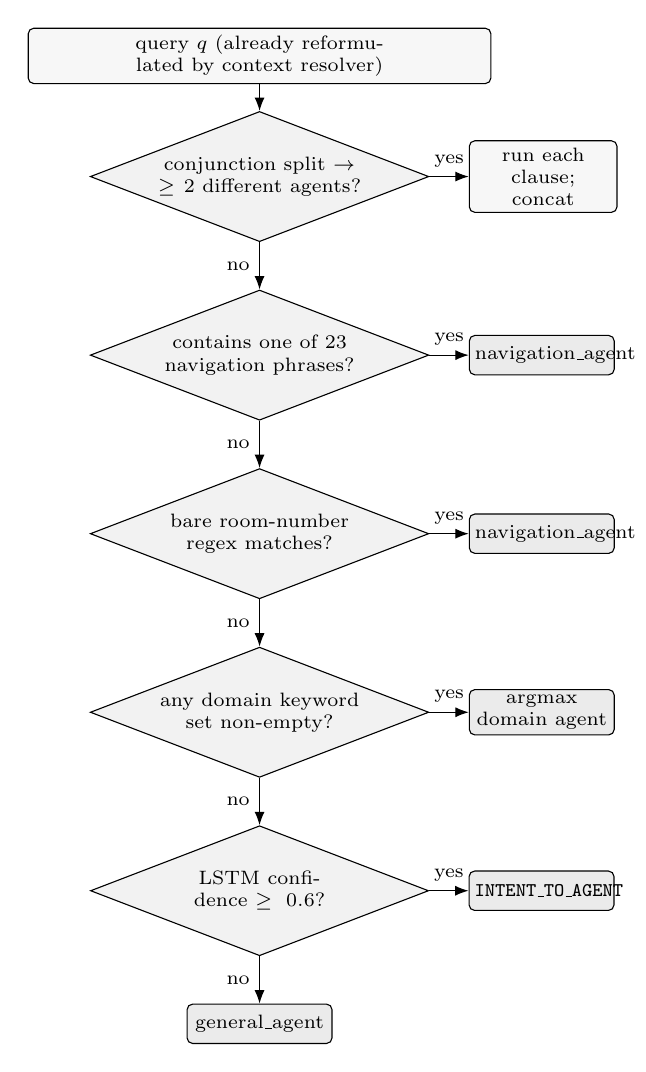
\begin{tikzpicture}[
  font=\scriptsize, node distance=3.4mm,
  b/.style={draw, rounded corners=2pt, align=center, text width=5.7cm, minimum height=5.5mm, inner sep=2.5pt, fill=black!3},
  d/.style={draw, diamond, aspect=2.6, align=center, inner sep=0pt, text width=3.0cm, fill=black!5},
  a/.style={draw, rounded corners=2pt, align=center, text width=1.7cm, minimum height=5mm, inner sep=2pt, fill=black!8},
  pf/.style={-{Latex[length=1.7mm]}}
]
\node[b] (q) {query $q$ (already reformulated by context resolver)};
\node[d, below=of q] (multi) {conjunction split $\to$ $\ge 2$ different agents?};
\node[d, below=6mm of multi] (nav) {contains one of 23 navigation phrases?};
\node[d, below=6mm of nav] (room) {bare room-number regex matches?};
\node[d, below=6mm of room] (kw) {any domain keyword set non-empty?};
\node[d, below=6mm of kw] (rnn) {LSTM confidence $\ge 0.6$?};
\node[a, right=5mm of nav] (na1) {navigation\_agent};
\node[a, right=5mm of room] (na2) {navigation\_agent};
\node[a, right=5mm of kw] (best) {argmax domain agent};
\node[a, right=5mm of rnn] (map) {\code{INTENT\_TO\_AGENT}};
\node[a, below=6mm of rnn] (gen) {general\_agent};
\node[b, right=5mm of multi, text width=1.7cm] (mrun) {run each clause; concat};

\draw[pf] (q)--(multi);
\draw[pf] (multi)-- node[left]{no} (nav);
\draw[pf] (multi)-- node[above]{yes} (mrun);
\draw[pf] (nav)-- node[left]{no} (room);
\draw[pf] (nav)-- node[above]{yes} (na1);
\draw[pf] (room)-- node[left]{no} (kw);
\draw[pf] (room)-- node[above]{yes} (na2);
\draw[pf] (kw)-- node[left]{no} (rnn);
\draw[pf] (kw)-- node[above]{yes} (best);
\draw[pf] (rnn)-- node[above]{yes} (map);
\draw[pf] (rnn)-- node[left]{no} (gen);
\end{tikzpicture}
\caption{Supervisor routing cascade. The first four tests are deterministic
substring/regex matches; the learned LSTM classifier is reached only when
none of them fire. Every decision is logged with its trigger.}
\label{fig:routing}
\end{figure}

\begin{table}[!t]
\centering
\caption{Query-Routing Approaches and the Implemented Hybrid.}
\label{tab:routing}
\footnotesize
\renewcommand{\arraystretch}{1.2}
\begin{tabular}{@{}p{1.55cm}p{1.55cm}p{1.55cm}p{2.2cm}@{}}
\toprule
\textbf{Property} & \textbf{Rule / keyword} & \textbf{Learned classifier} & \textbf{LLM router} \\
\midrule
Latency & negligible & ms (LSTM) & seconds \\
Cost & none & training only & per-query inference \\
Auditability & full (literal match) & partial (weights) & low \\
Unseen phrasing & misses & generalizes (if trained well) & robust \\
Cold-start data need & none & labeled corpus & none \\
Determinism & total & total at inference & low \\
\midrule
\multicolumn{4}{@{}p{7.6cm}@{}}{\textbf{Implemented:} deterministic phrase/keyword cascade
\emph{first}; trained LSTM ($12$ classes) consulted only on no-match, accepted
only if $P(\text{intent})\ge 0.6$; \code{general\_agent} otherwise. Combines
rule auditability with a learned safety net for uncovered phrasings.} \\
\bottomrule
\end{tabular}
\end{table}


The assistant is organized as a supervisor and five specialist agents ---
\code{admission\_agent}, \code{academic\_agent}, \code{facilities\_agent},
\code{navigation\_agent}, \code{general\_agent}. Here ``multi-agent''
denotes an intent-driven routing architecture~\cite{wooldridge2009mas}, not
concurrency and not an LLM-driven agent loop~\cite{wu2023autogen}: the
supervisor makes no factual claims, calls no LLM, and merely classifies and
dispatches.

\subsection{Specialist Agents}
All five agents are thin wrappers over one shared function,
\code{run\_specialist}, which executes the identical pipeline of
Section~\ref{sec:rag} (hybrid retrieval $\to$ rerank $\to$ context
selection $\to$ confidence $\to$ gated generation $\to$ grounding check
$\to$ curated fallback). What differs between agents is \emph{which queries
the supervisor sends them}, plus two agent-specific behaviors:
\code{navigation\_agent} first attempts two deterministic lookup paths
(a panorama-signage spatial knowledge store built from real main-building
room numbers, and a PostgreSQL entity resolver) and only falls through to
RAG on a miss, forcing confidence to $1.0$/HIGH on an exact structured
hit; and \code{general\_agent} is a pure pass-through appropriate for a
no-clear-domain fallback. No agent has a private retriever or model client;
none answers from parametric memory. This shared-pipeline discipline is an
explicit architectural invariant.

\subsection{Routing Algorithm}
\code{supervisor.classify} (Algorithm~\ref{alg:routing},
Fig.~\ref{fig:routing}) is a cascade evaluated in a fixed order:

\begin{enumerate}
\item \textbf{Navigation phrases.} A $23$-entry list of high-specificity
substrings (``where is'', ``how do i get to'', ``which floor'', ``take me
to'', ``panorama'', \dots) is checked first, because these are unambiguous
location signals even when the object contains another domain's keyword
(``Where is the CSE \emph{department}?'' is a location question).
\item \textbf{Bare room number.} A regular expression matching an optional
``room''/``room no.''/``\#'' prefix followed by a $2$--$4$ digit number and
an optional letter routes ``room 202'' to navigation regardless of
surrounding verbs.
\item \textbf{Domain keyword scoring.} Each of four domain keyword sets is
scored by the count of its members occurring in $q$; the highest-scoring
non-empty set wins.
\item \textbf{LSTM fallback.} \emph{Only} if steps 1--3 all fail, the
trained LSTM classifier is consulted; if $P(\text{intent}) \ge 0.6$, its
predicted class is mapped to an agent via a $12\!\to\!5$ dictionary,
otherwise \code{general\_agent} is chosen.
\end{enumerate}
Every decision returns a human-readable reason, and the supervisor logs
\code{"Routing decision: query=\%r -> agent=\%s (\%s)"} at \code{INFO}
level --- an explicit functional requirement for demonstrability and
auditability. This is a deliberate design choice against LLM-router
approaches (Table~\ref{tab:routing}): it costs no routing latency, needs no
per-query model call, and any decision can be explained from a single log
line.

\begin{algorithm}[!t]
\caption{Multi-Agent Query Routing}
\label{alg:routing}
\begin{algorithmic}[1]
\Require query $q$; navigation phrases $\mathcal{N}$; keyword sets $\{\mathcal{K}_a\}$;
threshold $\tau = 0.6$
\Ensure agent name(s) and reason
\State \textbf{// multi-domain pre-check}
\State $\Gamma \gets \textsc{SplitOnConjunction}(q)$ \Comment{on `` and '' / `` ; ''}
\If{$|\Gamma| \ge 2$ \textbf{and} $|\{\textsc{Classify}(\gamma) : \gamma \in \Gamma\}| \ge 2$}
  \State \textbf{return} $\{(\gamma, \textsc{Classify}(\gamma)) : \gamma \in \Gamma\}$ \Comment{run each, concatenate}
\EndIf
\State $\hat q \gets \text{lowercase}(q)$
\ForAll{$\pi \in \mathcal{N}$}
  \If{$\pi \subseteq \hat q$}\ \textbf{return} (\code{navigation\_agent}, ``phrase '$\pi$' '') \EndIf
\EndFor
\If{\textsc{RoomNumberRegex}$(q)$}\ \textbf{return} (\code{navigation\_agent}, ``bare room number'') \EndIf
\ForAll{agent $a$}\ $\sigma_a \gets |\{w \in \mathcal{K}_a : w \subseteq \hat q\}|$ \EndFor
\State $a^\star \gets \arg\max_a \sigma_a$
\If{$\sigma_{a^\star} > 0$}\ \textbf{return} $(a^\star,\ \text{``keywords ''} \dots)$ \EndIf
\State $(\iota, p) \gets \textsc{ClassifyIntentLSTM}(q)$ \Comment{Alg.~\ref{alg:lstm}}
\If{$\iota \ne \varnothing$ \textbf{and} $p \ge \tau$}
  \State \textbf{return} $(\textsc{IntentToAgent}[\iota],\ \text{``LSTM } \iota\ (p)\text{''})$
\EndIf
\State \textbf{return} (\code{general\_agent}, ``no rule matched; LSTM not confident'')
\end{algorithmic}
\end{algorithm}

\subsection{Multi-Domain Queries}
A thin opt-in layer splits a query on an explicit conjunction (`` and '',
`` ; '') and classifies each clause with the same \code{classify}. Only if
two or more clauses land on genuinely \emph{different} agents is the
multi-domain path taken: each clause is answered independently by its agent
and the answers are concatenated with no second LLM merge call. A query
like ``What is the admission process and what is the fee structure?''
splits into two clauses that both classify to \code{admission\_agent} and
therefore falls straight through to the ordinary single-agent path.

\subsection{LSTM Intent Classifier}
The classifier (Algorithm~\ref{alg:lstm}) is a compact recurrent
network~\cite{hochreiter1997lstm}:
\begin{align}
\mathbf{x}_t &= \mathbf{E}\,\text{onehot}(w_t), \quad \mathbf{E}\in\mathbb{R}^{|\mathcal{V}|\times 32},\\
(\mathbf{h}_t,\mathbf{c}_t) &= \mathrm{LSTM}(\mathbf{x}_t, \mathbf{h}_{t-1}, \mathbf{c}_{t-1}), \quad \mathbf{h}_t\in\mathbb{R}^{32},\\
\mathbf{z} &= \mathbf{W}\,\mathrm{dropout}_{0.2}(\mathbf{h}_{T}) + \mathbf{b}, \quad \mathbf{W}\in\mathbb{R}^{12\times 32},\\
P(\text{class} = j \mid q) &= \mathrm{softmax}(\mathbf{z})_j,
\end{align}
where $w_1{:}w_T$ are the query's lowercase alphanumeric tokens,
$\mathbf{h}_T$ is the final hidden state after a packed sequence pass, and
the classifier head produces logits over $12$ classes. Vocabulary
$\mathcal{V}$ has $283$ entries (plus \code{<pad>}/\code{<unk>}); the same
minimal tokenizer as BM25 is used so that room numbers and acronyms are not
fragmented. Inference applies \code{softmax} and returns the arg-max class
with its probability; if artifacts are missing the classifier returns
$(\varnothing, 0)$ and the supervisor treats that as ``no opinion.''

\begin{algorithm}[!t]
\caption{LSTM Intent Classification Pipeline}
\label{alg:lstm}
\begin{algorithmic}[1]
\Require query $q$; vocab $\mathcal{V}$; trained params $(\mathbf{E},\text{LSTM},\mathbf{W},\mathbf{b})$; classes $\mathcal{I}$ ($|\mathcal{I}|{=}12$)
\Ensure $(\text{intent},\ \text{probability})$
\If{artifacts absent} \textbf{return} $(\varnothing,\ 0)$ \EndIf
\State $[w_1,\dots,w_T] \gets \textsc{Tokenize}(q)$ \Comment{\code{[a-z0-9]+}}
\If{$T = 0$} \textbf{return} $(\varnothing,\ 0)$ \EndIf
\State $\text{ids} \gets [\,\mathcal{V}.\text{get}(w_t, \langle\text{unk}\rangle)\,]_{t=1}^{T}$
\State $\mathbf{z} \gets \textsc{IntentLSTM}(\text{ids},\ \text{lengths}{=}T)$ \Comment{embed $\to$ pack $\to$ LSTM $\to$ dropout $\to$ linear}
\State $\mathbf{p} \gets \mathrm{softmax}(\mathbf{z})$;\ $j^\star \gets \arg\max_j p_j$
\State \textbf{return} $(\mathcal{I}[j^\star],\ p_{j^\star})$
\end{algorithmic}
\end{algorithm}

\subsection{Training and Its Limitations}
Training uses $168$ hand-authored synthetic utterances (the module's own
docstring labels them ``not logged real user queries''), a seeded $80/20$
split ($134$ train, $34$ validation), Adam ($\text{lr}=0.01$, weight decay
$10^{-3}$), cross-entropy loss, $150$ epochs, and best-validation-accuracy
early stopping. The saved checkpoint reports \textbf{training accuracy
$1.00$ and validation accuracy $0.529$} --- a textbook overfitting
signature on a tiny synthetic set~\cite{goodfellow2016deep}. An independent
re-evaluation reproduced exactly $0.529$ and produced the per-class
breakdown in Section~\ref{sec:results}: four of the twelve classes have
$F_1 = 0$. \textbf{We therefore make no generalization claim for this
classifier.} Its role is strictly a fallback signal behind the
deterministic rules, and even in that role it is gated at $P \ge 0.6$.
The $12$ fine-grained classes (e.g.\ separating \code{ROOM\_LOCATION} from
\code{DEPARTMENT\_LOCATION}) collapse onto the $5$ agents; the finer labels
exist so the classifier reports a useful intent even though several map to
the same agent.

\subsection{Design Rationale}
The deterministic-first design is justified by four constraints from
Section~\ref{sec:problem}: (i)~zero routing latency matters when the
generation step already costs seconds; (ii)~the deterministic rules are
zero-false-negative for the phrasings they cover and were not tuned to pass
any particular test; (iii)~every routing decision must be explainable from
logs; and (iv)~no labeled routing corpus exists to train a primary
classifier on. The LSTM adds coverage for paraphrases outside the keyword
lists (``What can I study here?'' contains no course keyword) without
making routing confidence-dependent for the common case.

\section{Graph-Based Campus Navigation}
\label{sec:nav}
\begin{figure}[!t]
\centering
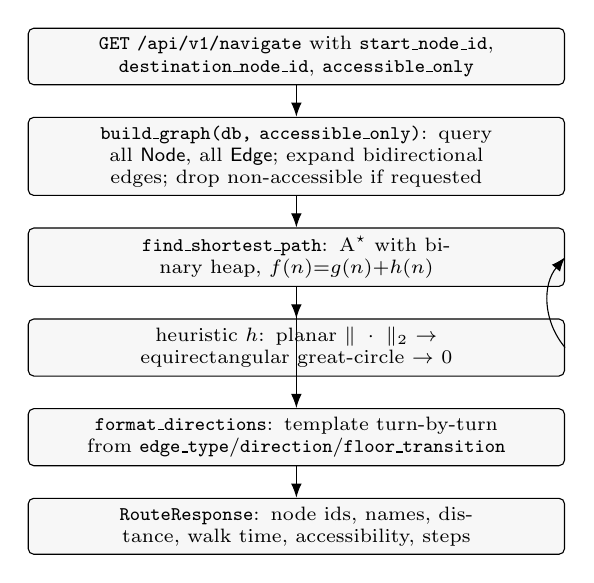
\begin{tikzpicture}[
  font=\scriptsize, node distance=4mm,
  b/.style={draw, rounded corners=2pt, align=center, text width=6.6cm, minimum height=6mm, inner sep=3pt, fill=black!3},
  pf/.style={-{Latex[length=1.8mm]}}
]
\node[b] (req) {\code{GET /api/v1/navigate} with \code{start\_node\_id}, \code{destination\_node\_id}, \code{accessible\_only}};
\node[b, below=of req] (build) {\code{build\_graph(db, accessible\_only)}: query all \textsf{Node}, all \textsf{Edge}; expand bidirectional edges; drop non-accessible if requested};
\node[b, below=of build] (astar) {\code{find\_shortest\_path}: A$^{\star}$ with binary heap, $f(n){=}g(n){+}h(n)$};
\node[b, below=of astar] (heur) {heuristic $h$: planar $\|\cdot\|_2$ $\rightarrow$ equirectangular great-circle $\rightarrow$ $0$};
\node[b, below=of heur] (fmt) {\code{format\_directions}: template turn-by-turn from \code{edge\_type}/\code{direction}/\code{floor\_transition}};
\node[b, below=of fmt] (resp) {\code{RouteResponse}: node ids, names, distance, walk time, accessibility, steps};
\draw[pf] (req)--(build); \draw[pf] (build)--(astar); \draw[pf] (astar)-- (heur);
\draw[pf] (heur.east) to[bend left=40] (astar.east);
\draw[pf] (astar)--(fmt); \draw[pf] (fmt)--(resp);
\end{tikzpicture}
\caption{A$^{\star}$ navigation pipeline. The graph is rebuilt from the live
relational schema on every request; there is no persistent in-process graph
cache and (currently) no front-end consumer of the endpoint.}
\label{fig:astar}
\end{figure}

\begin{table}[!t]
\centering
\caption{Campus Navigation Approaches and the Implemented Choice.}
\label{tab:nav}
\footnotesize
\renewcommand{\arraystretch}{1.2}
\begin{tabular}{@{}p{1.7cm}p{2.0cm}p{1.5cm}p{1.9cm}@{}}
\toprule
\textbf{Approach} & \textbf{Optimality} & \textbf{Needs coords} & \textbf{Role in \system{}} \\
\midrule
BFS / DFS traversal & unweighted only & no & not used \\
Dijkstra \cite{dijkstra1959note} & optimal (non-neg.\ weights) & no & single-source nearest-facility queries \\
A$^{\star}$ \cite{hart1968astar} & optimal if $h$ admissible & optional & primary point-to-point pathfinder \\
GPS turn-by-turn & n/a & yes (outdoor) & built, then removed from codebase \\
Panorama link traversal & n/a & no & the tour (Section~\ref{sec:tour}), not routing \\
\midrule
\multicolumn{4}{@{}p{7.6cm}@{}}{\textbf{Implemented:} A$^{\star}$ with a three-tier
degrading heuristic; at the zero tier it is provably identical to Dijkstra,
so a single code path covers both. Back end complete; no UI consumer.} \\
\bottomrule
\end{tabular}
\end{table}


The wayfinding engine (\code{backend/app/navigation/}) computes shortest
walking routes over the campus graph; Table~\ref{tab:nav} situates the
implemented A$^{\star}$ choice among alternative routing approaches. It has
been intact and unit-tested since an early project phase; a later scope
revision removed its natural-language chat entry point but kept the engine,
which is now exposed only through \code{GET /api/v1/navigate} and internal
nearest-panorama lookups. It currently has \textbf{no front-end consumer} --- a
previously built map UI with GPS turn-by-turn guidance was deliberately
removed from the codebase.

\subsection{Database-Backed Graph Construction}
The navigation graph is \emph{not} stored as a file; it is rebuilt on every
request from the live relational schema (Algorithm~\ref{alg:graphbuild}).
\code{build\_graph} loads all $\textsf{Node}$ rows and all $\textsf{Edge}$
rows (filtering out non-accessible edges when \code{accessible\_only} is
set), then constructs an adjacency list $A: \mathrm{id} \to
[\textsf{GraphEdge}]$ in which each directed edge $(u,v)$ contributes
$A[u] \mathrel{+}= (v, \text{dist}, e)$ and, if
\code{is\_bidirectional}, also $A[v] \mathrel{+}= (u, \text{dist}, e)$.

\begin{algorithm}[!t]
\caption{Database-Backed Graph Construction}
\label{alg:graphbuild}
\begin{algorithmic}[1]
\Require DB session; flag \code{accessible\_only}
\Ensure \code{CampusGraph}$(A,\ \text{nodesById})$
\State $\text{nodesById} \gets \{\, n.\text{id} \mapsto n : n \in \textsc{SelectAll}(\textsf{Node}) \,\}$
\State $Q \gets \textsc{Select}(\textsf{Edge})$;\ \textbf{if} \code{accessible\_only} \textbf{then} $Q \gets Q\ \textbf{where}\ e.\text{accessible}$
\State $A \gets \{\, i \mapsto [\,] : i \in \text{nodesById} \,\}$
\ForAll{$e \in Q$}
  \State $A[e.\text{src}] \mathrel{+}= (e.\text{tgt},\ e.\text{distance},\ e)$
  \If{$e.\text{is\_bidirectional}$}\ $A[e.\text{tgt}] \mathrel{+}= (e.\text{src},\ e.\text{distance},\ e)$ \EndIf
\EndFor
\State \textbf{return} \code{CampusGraph}$(A,\ \text{nodesById})$
\end{algorithmic}
\end{algorithm}

Using the normalized relational schema as the live source of truth has
three benefits for this project: the graph is always consistent with the
tour and the minimap (which read the same tables); edits go through the
same CRUD/migration tooling as every other campus fact; and accessibility
filtering is a query predicate rather than a separate data set. The cost is
that each route request pays an $O(|V| + |E|)$ rebuild ($180 + 325$ rows);
Section~\ref{sec:eval} proposes measuring whether this warrants a cache.

\subsection{A$^{\star}$ Shortest Path}
The search (Algorithm~\ref{alg:astar}, Fig.~\ref{fig:astar}) is textbook
A$^{\star}$~\cite{hart1968astar,russell2020aima} with a binary heap. It
expands the node minimizing
\begin{equation}
f(n) \;=\; g(n) + h(n, t),
\label{eq:fn}
\end{equation}
where $t$ is the goal node. The accumulated cost uses the stored edge
distance,
\begin{equation}
g(v) \;=\; g(u) + \mathrm{dist}(u,v), \qquad (u,v) \in E,
\label{eq:gn}
\end{equation}
and $\mathrm{dist}(u,v)$ is the \code{Edge.distance} column (a surveyed or
authored float, not derived from coordinates). Path reconstruction walks a
\code{came\_from} map from goal to start. The equal-node fast path returns
immediately; a start or goal absent from the graph raises a typed
no-path error.

\begin{algorithm}[!t]
\caption{A$^{\star}$ Campus Pathfinding}
\label{alg:astar}
\begin{algorithmic}[1]
\Require graph $(A, \text{nodesById})$; start $s$; goal $t$
\Ensure path node ids, edge list, total distance
\If{$s \notin \text{nodesById}$ \textbf{or} $t \notin \text{nodesById}$}\ \textbf{raise} NoPath \EndIf
\If{$s = t$}\ \textbf{return} $([s],\ [\,],\ 0)$ \EndIf
\State open $\gets$ min-heap $\{(0, s)\}$;\ $g[s] \gets 0$;\ visited $\gets \emptyset$;\ came $\gets \{\}$
\While{open $\ne \emptyset$}
  \State $(\cdot,u) \gets \textsc{HeapPop}(\text{open})$
  \If{$u \in$ visited}\ \textbf{continue} \EndIf
  \State visited $\gets$ visited $\cup \{u\}$
  \If{$u = t$}\ \textbf{return} \textsc{Reconstruct}(came, $s$, $t$, $g[t]$) \EndIf
  \ForAll{$(v, w, e) \in A[u]$}
    \State $g' \gets g[u] + w$
    \If{$g' < g.\text{get}(v, \infty)$}
       \State $g[v] \gets g'$;\ came$[v] \gets (u, e)$
       \State \textsc{HeapPush}$\big(\text{open},\ (g' + h(\text{nodesById}[v], \text{nodesById}[t]),\ v)\big)$
    \EndIf
  \EndFor
\EndWhile
\State \textbf{raise} NoPath
\end{algorithmic}
\end{algorithm}

\subsection{Three-Tier Degrading Heuristic}
The heuristic adapts to whatever spatial information the two nodes share:
\begin{equation}
h(a,b) =
\begin{cases}
\sqrt{(a_x - b_x)^2 + (a_y - b_y)^2}, & \text{planar coords on both,}\\[1.2ex]
\sqrt{(\Delta\!X)^2 + (\Delta\!Y)^2}, & \text{geographic coords on both,}\\[1.2ex]
0, & \text{otherwise,}
\end{cases}
\label{eq:heur}
\end{equation}
with the equirectangular approximation
\begin{align}
\Delta\!X &= (a_{\text{lon}} - b_{\text{lon}})\cdot 111{,}320 \cdot \cos\!\Big(\tfrac{a_{\text{lat}} + b_{\text{lat}}}{2}\Big),\\
\Delta\!Y &= (a_{\text{lat}} - b_{\text{lat}})\cdot 110{,}540,
\end{align}
adequate at campus scale. All three tiers are \emph{admissible}: tiers~1
and~2 are straight-line lower bounds on any walk, and $h \equiv 0$ trivially
never overestimates. At tier~3 the priority in~\eqref{eq:fn} reduces to
$f(n) = g(n)$, i.e.\ the search \emph{is} Dijkstra's
algorithm~\cite{dijkstra1959note}. A separate \code{single\_source\_distances}
routine runs plain Dijkstra for nearest-facility queries (nearest room,
nearest panorama), where there is no single fixed goal for a heuristic to
aim at. Because all building \code{latitude}/\code{longitude} values and
most node coordinates are currently null, the system in its present state
runs predominantly at tier~3 (Dijkstra behavior); this is correct, just
uninformed, and improves automatically as real coordinates are surveyed.

\subsection{Turn-by-Turn Directions}
\code{format\_directions} converts the node/edge path into template-based
steps with no LLM involvement: a movement verb keyed on \code{edge\_type}
(``Walk through the corridor'', ``Take the stairs'', ``Take the
elevator''), a turn cue keyed on the relative \code{direction} enumeration
(``Turn left.''), a floor-name cue on floor-transition edges, and, on the
final step into a room, a ``\emph{Room X} is on your left/right'' cue. The
\code{RouteResponse} carries the ordered node ids and names, total
distance, an estimated walk time (summed per-edge \code{walking\_time}, or
distance $/\,1.2\,\text{m\,s}^{-1}$), and a whole-path accessibility flag
(true iff every edge on the path is wheelchair-passable, independent of
whether accessible-only routing was requested).

\section{Voice Interaction}
\label{sec:voice}
\begin{figure}[!t]
\centering
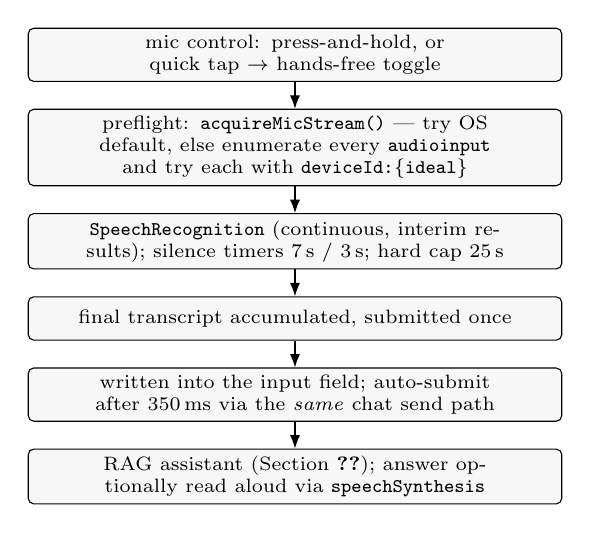
\begin{tikzpicture}[
  font=\scriptsize, node distance=3.4mm,
  b/.style={draw, rounded corners=2pt, align=center, text width=6.6cm, minimum height=5.5mm, inner sep=2.5pt, fill=black!3},
  pf/.style={-{Latex[length=1.7mm]}}
]
\node[b] (press) {mic control: press-and-hold, or quick tap $\to$ hands-free toggle};
\node[b, below=of press] (pre) {preflight: \code{acquireMicStream()} --- try OS default, else enumerate every \code{audioinput} and try each with \code{deviceId:\{ideal\}}};
\node[b, below=of pre] (rec) {\code{SpeechRecognition} (continuous, interim results); silence timers $7$\,s / $3$\,s; hard cap $25$\,s};
\node[b, below=of rec] (tx) {final transcript accumulated, submitted once};
\node[b, below=of tx] (send) {written into the input field; auto-submit after $350$\,ms via the \emph{same} chat send path};
\node[b, below=of send] (rag) {RAG assistant (Section~\ref{sec:rag}); answer optionally read aloud via \code{speechSynthesis}};
\draw[pf] (press)--(pre); \draw[pf] (pre)--(rec); \draw[pf] (rec)--(tx);
\draw[pf] (tx)--(send); \draw[pf] (send)--(rag);
\end{tikzpicture}
\caption{Voice-to-RAG interaction pipeline. Speech-to-text is
browser-native and never contacts the back end directly; text-to-speech is
optional and browser-native. Voice-navigation command parsing is not
implemented.}
\label{fig:voice}
\end{figure}


Voice input is provided entirely in the browser through the Web Speech API,
consistent with the constraint of incurring no server-side voice cost
(Fig.~\ref{fig:voice}). There is \emph{zero} voice code in the back end.

\subsection{Speech-to-Text}
The \code{useSpeechRecognition} hook wraps \code{SpeechRecognition} /
\code{webkitSpeechRecognition}. Feature detection runs post-mount to avoid a
server/client hydration mismatch. Recognition runs in continuous mode with
interim results so a brief mid-sentence pause does not end the session
early; final fragments are accumulated and submitted exactly once, when
recognition ends (user release, a $3$-second post-speech silence timeout, a
$7$-second initial-silence timeout, or a $25$-second hard cap). Error codes
are mapped to actionable messages distinguishing permission denial, no
speech, no microphone, and an engine that cannot open the OS default input.

A microphone-acquisition routine, \code{acquireMicStream}, first attempts
an unconstrained \code{getUserMedia(\{audio:true\})}; on
\code{NotFoundError}, \code{OverconstrainedError}, or \code{NotReadableError}
it enumerates every real \code{audioinput} device and tries each with
\code{deviceId:\{ideal\}}. This specifically addresses the case where the
operating system's default communication device is stale (e.g.\ a
disconnected Bluetooth headset) while the built-in microphone is present
and usable as a non-default device. It never retries on a permission
denial. A development-only diagnostic panel reports device counts before
and after permission, track state, and which acquisition step succeeded.

On a successful transcript, the text is written into the chat input and
auto-submitted after $350$\,ms through the \emph{same} send path as typed
input --- voice never talks to the back end directly. Recognition language
follows the selected UI language.

\subsection{Text-to-Speech}
An optional ``read answers aloud'' toggle uses \code{speechSynthesis}. The
hook ranks available voices (preferring a regional and then a
network/neural voice, never requiring one), strips markdown and citation
artifacts before speaking, and splits the answer into moderate-length
utterances for natural pacing. This affects only spoken output; the
displayed text is untouched.

\subsection{What Is Not Implemented}
There is no voice-navigation command parsing: a transcript such as ``take
me to the library'' is passed to the chat pipeline as an ordinary query and
is \emph{not} intercepted as a navigation intent. There are no server-side
speech endpoints. These omissions are consistent with the browser-only
design intent; they are narrower in scope than an aspirational ``voice
navigation'' feature.

\section{Implementation and Technology Stack}
\label{sec:impl}
\begin{table}[!t]
\centering
\caption{Implementation Technology Stack (Versions as Pinned in the Repository).}
\label{tab:stack}
\footnotesize
\renewcommand{\arraystretch}{1.15}
\begin{tabular}{@{}p{1.9cm}p{2.6cm}p{2.7cm}@{}}
\toprule
\textbf{Layer} & \textbf{Technology} & \textbf{Role} \\
\midrule
Front end & Next.js 15.5, React 19, TypeScript 5.9 & App-Router SPA, strict typing \\
& Tailwind CSS 3.4, Framer Motion 11 & styling, animation \\
& TanStack Query 5, Zustand 4.5 & server / client state \\
& \code{pannellum-react} 1.3 & 360$^{\circ}$ viewer \\
& \code{@vis.gl/react-google-maps} 1.9 & satellite map \\
& Web Speech API & browser STT / TTS \\
& custom dictionary + hook & EN/KN/HI UI translation \\
\midrule
API & FastAPI $\ge$0.115, Pydantic 2 & async framework, sync chat handler \\
\midrule
Data & PostgreSQL 16, SQLAlchemy 2 (sync), Alembic & campus schema, sessions, 14 migrations \\
& ChromaDB $\ge$0.5 (\code{PersistentClient}) & vector store, HNSW cosine \\
\midrule
AI / RAG & LangChain + \code{langchain-ollama} & orchestration wrapper \\
& Ollama, Llama~3.2 & local LLM (generation, translation) \\
& \code{sentence-transformers}, \code{all-MiniLM-L6-v2} & 384-d embeddings \\
& \code{rank\_bm25} (BM25Okapi) & lexical retrieval \\
& scikit-learn \code{SVR} & reranker (implemented, untrained) \\
& PyTorch $\ge$2.0 LSTM & intent classifier \\
& BeautifulSoup4, \code{pypdf} & KB source acquisition \\
\midrule
Packaging & Docker Compose & 4 services; no cache/queue \\
\bottomrule
\end{tabular}
\end{table}


\system{} is implemented as a Dockerized multi-service application
(Table~\ref{tab:stack}). This section records implementation decisions that
affect the system's behavior and that a reader reproducing the work needs
to know.

\subsection{Front End}
The front end is a Next.js~15 App-Router application in strict TypeScript.
Business logic is kept out of route files; the \code{lib}/\code{api} layer
is the only place HTTP is issued; three Zustand stores hold cross-component
state, with the chat store persisted to \code{localStorage} so a
conversation and its session id survive a reload. The 360$^{\circ}$ viewer
is \code{pannellum-react}, dynamically imported with \code{ssr:false}. UI
translation for English, Kannada, and Hindi is a hand-maintained lookup
dictionary keyed on the English source string, deliberately not a
full i18n framework, because the static-string surface is small and a
missing key degrades gracefully to English.

\subsection{Back End}
The API is FastAPI~\cite{ramirez2018fastapi} with Pydantic response models
on every route and a non-wildcard CORS origin list. The chat route is synchronous by design (see
Section~\ref{sec:architecture}); the tour and CRUD routes are likewise
synchronous, matching the codebase's actual prevailing convention rather
than an aspirational async-everywhere rule. The RAG/agent code in
\code{scripts/ai/} is imported into the API process through a
\code{sys.path} insertion --- a documented, deliberate deviation from the
repository's folder convention that avoids duplicating a six-stage,
independently tested pipeline inside \code{backend/app/}.

\subsection{Model Serving and Concurrency}
Generation uses Ollama-served Llama~3.2 (note: the model actually pulled
and used is \code{llama3.2}, not the \code{llama3} that a stale
configuration default names). Both the embedding model and the BM25 index
are process singletons, and both --- together with the Ollama model --- are
explicitly warmed at server startup, because a cold first request loaded
the encoder and tokenized/indexed $1{,}507$ chunks inline and exceeded the
front-end's $10$-second HTTP timeout. Concurrent Ollama calls are
serialized by a semaphore (default width $1$) after two simultaneous
requests were measured degrading to $17$\,s and $45$\,s on the CPU-only
host (Section~\ref{sec:results}).

\subsection{Persistence and Migrations}
PostgreSQL holds the campus schema and chat-session history; SQLAlchemy is
used synchronously with the \code{psycopg2} driver. Fourteen Alembic
revisions define the schema. Session writes are best-effort: a database
hiccup degrades conversation \emph{persistence} (loss of follow-up
continuity for one exchange) but never the answer itself.

\subsection{Deployment}
Docker Compose defines exactly four services --- \code{frontend},
\code{backend}, \code{db} (\code{postgres:16-alpine}), and \code{ollama}
--- with no cache or message-queue service. There is no hosted-deployment
configuration; the only supported deployment path is local Compose. The CI
workflow is a placeholder that runs no lint, type-check, or test step,
although the repository configures \code{ruff}/\code{black}/\code{mypy}/
\code{pytest} and the front end has lint and type-check scripts. The
automated test suites (\code{tests/backend}, \code{tests/frontend},
\code{tests/e2e}) are currently empty placeholders; testing to date has
been via standalone per-stage scripts.

\subsection{Security Posture}
There is no authentication on any endpoint, including the CRUD routes that
can mutate campus data; the chat-session model carries no user concept.
CORS origins are restricted but methods and headers are wildcarded. Raw
user chat messages are logged verbatim at \code{INFO} level, which is a
deviation from the project's own PII-logging guidance and should be
addressed before any real deployment. Dev-only authoring panels are gated
only by build-time client flags, not server-side authorization. These
issues are enumerated so they are not mistaken for solved problems.

\section{Experimental Methodology and Proposed Evaluation Protocol}
\label{sec:eval}
\begin{table*}[!t]
\centering
\caption{Proposed Evaluation Protocol. None of These Experiments Has Been
Run; They Are Specified Here as the Required Next Step, Not Reported as
Results.}
\label{tab:evalprotocol}
\footnotesize
\renewcommand{\arraystretch}{1.25}
\begin{tabular}{@{}p{2.5cm}p{3.4cm}p{4.0cm}p{4.7cm}@{}}
\toprule
\textbf{Experiment} & \textbf{Metrics} & \textbf{Data / apparatus} & \textbf{Baselines / conditions} \\
\midrule
E1 Retrieval quality &
P@1, P@3, P@5, R@5, MRR, nDCG@10 \cite{jarvelin2002ndcg} &
$\ge$150 institution queries with graded relevance judgments over the
$1{,}507$-chunk corpus &
BM25 only; dense only; hybrid $\lambda\!\in\!\{0.3,0.5,0.6,0.7\}$; effect of
query expansion \\

E2 Reranker ablation &
$\Delta$ nDCG@5, P@5 vs.\ no rerank &
E1 query set + feature vectors &
no rerank; heuristic (Eq.~\eqref{eq:rerank}); trained SVR (after labeling);
weight sensitivity \\

E3 Intent classification &
accuracy, macro/weighted $F_1$, per-class $F_1$, $12{\times}12$ confusion &
$\ge$600 real logged queries, human-labeled, stratified split &
current LSTM (as-is); LSTM retrained on real data; keyword-rule router;
zero-shot LLM classifier \\

E4 Answer faithfulness &
faithfulness, answer relevancy, context relevancy \cite{es2024ragas};
manual hallucination rate; citation correctness &
$\ge$120 questions (in-domain / out-of-scope / ambiguous); LLM judge +
2 human raters, report $\kappa$ &
full pipeline; ablate confidence gate; ablate grounding check; ablate both \\

E5 Confidence calibration &
coverage, refusal rate, hallucination rate, answered-accuracy vs.\
$(\theta_{\text{MED}}, \theta_{\text{HIGH}})$; reliability diagram, ECE &
E4 question set with correctness labels &
sweep $\theta$ on a grid; with vs.\ without LSTM $P(\text{intent})$ in
Eq.~\eqref{eq:conf} \\

E6 Pathfinding &
path length, wall-clock, expanded-node count vs.\ graph size &
the $180$/$325$ graph + synthetically scaled graphs; synthetic coordinates
for tier-1/2 heuristic &
A$^{\star}$ (3 heuristic tiers) vs.\ Dijkstra; cached vs.\ rebuilt graph \\

E7 Tour traversal &
cross-floor transition success, guided-tour completion rate, orientation
continuity error, interaction errors &
scripted traversals over all $6$ floor buckets; fault-injected corrupt
graphs &
manual vs.\ guided; with vs.\ without cycle guard \\

E8 Usability &
task completion rate, time-on-task, SUS, satisfaction, trust &
$\ge$20 participants (prospective students), $6$ tasks spanning QA + tour +
(future) routing &
\system{} vs.\ institution website + PDF brochures \\
\bottomrule
\end{tabular}
\end{table*}


The current artifact contains \emph{no} formal evaluation pipeline: there
are no retrieval precision/recall figures, no answer-faithfulness scores,
no reranker comparison, no full intent-classifier confusion matrix beyond
the one reproduced in Section~\ref{sec:results}, no load-test results, no
pathfinding benchmark, and no user study. Rather than fabricate any of
these, this section specifies exactly how each should be measured. The
protocol is summarized in Table~\ref{tab:evalprotocol}; the subsections
below give the design detail. We distinguish \emph{implementation metrics}
(Table~\ref{tab:counts}, already measured) from \emph{experimental
performance metrics} (E1--E8 below, not yet measured).

\subsection{E1 --- Retrieval Quality}
\emph{Objective:} test whether hybrid fusion~\eqref{eq:fusion} outperforms
its components on this corpus, and whether $\lambda = 0.6$ is well chosen.
\emph{Apparatus:} construct a query set of at least $150$ realistic
institution questions (admissions, academics, facilities, campus info,
out-of-scope) and, for each, human-annotate graded relevance for the pooled
top-$k$ of BM25, dense, and hybrid retrieval, following BEIR-style pooling
practice~\cite{thakur2021beir}. \emph{Metrics:} precision@$\{1,3,5\}$,
recall@$5$, MRR, and nDCG@$10$~\cite{jarvelin2002ndcg}. \emph{Conditions:}
BM25 only; dense only; hybrid at
$\lambda \in \{0.3, 0.5, 0.6, 0.7\}$; hybrid with and without query
expansion. \emph{Expected finding form:} ``hybrid at $\lambda=x$ achieves
nDCG@10 $= y$, a $\Delta$ of $z$ over the stronger single method
($p < 0.05$, paired bootstrap).'' No such claim is made here.

\subsection{E2 --- Reranker Ablation}
\emph{Objective:} quantify the heuristic reranker's contribution and, once
E1 has produced relevance labels, train and evaluate the currently-untrained
SVR. \emph{Conditions:} no reranking; the four-feature heuristic of
Eq.~\eqref{eq:rerank}; $\varepsilon$-SVR trained on E1 labels; a sensitivity
sweep of the four heuristic weights. \emph{Metrics:} $\Delta$nDCG@$5$ and
$\Delta$P@$5$ against the no-rerank baseline. Until the SVR is trained, no
number for it may be reported.

\subsection{E3 --- Intent Classification}
\emph{Objective:} measure generalization on \emph{real} queries, not the
synthetic seed set. \emph{Apparatus:} sample at least $600$ queries from
the accumulated chat logs, have two annotators label them into the $12$
classes (report inter-annotator $\kappa$), and split stratified by class.
\emph{Conditions:} the current LSTM as-is; the LSTM retrained on the real
labeled data; the deterministic keyword router alone; a zero-shot LLM
classifier. \emph{Metrics:} accuracy, macro and weighted $F_1$, per-class
$F_1$, and the full $12{\times}12$ confusion matrix. \emph{Framing:} the
current $0.529$ validation accuracy on $34$ synthetic examples
(Section~\ref{sec:results}) is explicitly \emph{not} a generalization
estimate; E3 is what would produce one.

\subsection{E4 --- Answer Faithfulness and Relevancy}
\emph{Objective:} measure whether generated answers are entailed by their
cited context and whether the safeguards matter. \emph{Apparatus:} a fixed
question set of at least $120$ items spanning in-domain, out-of-scope, and
deliberately ambiguous queries; scoring by an LLM judge for faithfulness,
answer relevancy, and context relevancy~\cite{es2024ragas}, cross-checked
by two human raters on a subset (report agreement); a manually adjudicated
hallucination rate; and citation-correctness (does each cited source
actually support the answer). \emph{Ablations:} full pipeline; remove the
confidence gate; remove the post-generation grounding check; remove both.
\emph{Correct-refusal behavior:} for out-of-scope and ambiguous items,
score whether the system refused or asked a clarifying question rather than
answering. This is the single highest-value missing measurement for a
results section.

\subsection{E5 --- Confidence-Threshold Calibration}
\emph{Objective:} replace the nine-query threshold derivation
(Table~\ref{tab:confsample}) with a statistically sized calibration.
\emph{Apparatus:} the E4 question set with per-item correctness labels.
\emph{Analysis:} sweep $(\theta_{\text{MED}}, \theta_{\text{HIGH}})$ on a
grid and plot coverage, refusal rate, hallucination rate, and
answered-accuracy; produce a reliability diagram and report expected
calibration error. \emph{Additional condition:} repeat with the LSTM's
$P(\text{intent})$ actually supplied to Eq.~\eqref{eq:conf} (closing the
implementation gap noted in Section~\ref{sec:rag}), to test whether the
intent term improves separation.

\subsection{E6 --- Pathfinding Performance}
\emph{Objective:} characterize A$^{\star}$ on the live graph and against
Dijkstra. \emph{Apparatus:} the $180$-node/$325$-edge graph plus
synthetically scaled graphs (up to $10^4$ nodes) and synthetic node
coordinates so tiers~1 and~2 of the heuristic~\eqref{eq:heur} are
exercised. \emph{Metrics:} route length (should be identical to Dijkstra,
verifying optimality), wall-clock time, and expanded-node count as a
function of graph size and heuristic tier; the marginal cost of rebuilding
the graph per request vs.\ caching it.

\subsection{E7 --- Tour Traversal Correctness}
\emph{Objective:} verify the scene-graph mechanisms. \emph{Apparatus:}
scripted traversals covering every one of the six floor buckets and every
cross-floor boundary; fault-injected corrupt graphs (self-loops, dangling
tails). \emph{Metrics:} cross-floor transition success rate, guided-tour
completion rate, camera-orientation continuity error at transitions
(deviation from the Street-View heading-preservation rule), and interaction
errors; verification that the cycle guard aborts to \emph{error} rather
than looping.

\subsection{E8 --- Usability}
\emph{Objective:} measure whether the integrated system helps real users.
\emph{Apparatus:} at least $20$ prospective-student participants performing
six tasks that each require both propositional and spatial information
(e.g.\ ``find which floor the Power System Simulation Lab is on and view
it''). \emph{Comparison:} \system{} vs.\ the institution's website plus PDF
brochures. \emph{Metrics:} task completion rate, time-on-task, System
Usability Scale, satisfaction, and a trust item (``I would rely on this
system's answers''). \emph{Analysis:} paired tests with effect sizes.

\subsection{Reproducibility Requirements}
Any reported result must also record: exact hardware (CPU/GPU, RAM, whether
Ollama ran on CPU or GPU); the Llama~3.2 quantization and Ollama version;
the corpus snapshot (chunk count and manifest hash); and the random seeds.
The current paper reports none of these because no experiment has been run.

\section{Current Implementation Measurements and Discussion}
\label{sec:results}
\begin{table}[!t]
\centering
\caption{Intent Classifier: Measured Per-Class Metrics on the Reconstructed
$34$-Example Validation Split (Seed $42$). Overall Accuracy $0.5294$;
Macro $F_1$ $0.4042$; Weighted $F_1$ $0.4869$.}
\label{tab:lstmperclass}
\footnotesize
\renewcommand{\arraystretch}{1.12}
\begin{tabular}{@{}lrrrr@{}}
\toprule
\textbf{Class} & \textbf{Prec.} & \textbf{Rec.} & \textbf{$F_1$} & \textbf{Supp.} \\
\midrule
ADMISSIONS          & 1.000 & 0.200 & 0.333 & 5 \\
COURSES             & 0.400 & 0.500 & 0.444 & 4 \\
DEPARTMENTS         & 0.667 & 1.000 & 0.800 & 2 \\
ACADEMICS           & 0.667 & 1.000 & 0.800 & 2 \\
FACILITIES          & 0.600 & 1.000 & 0.750 & 3 \\
ROOM\_LOCATION      & 1.000 & 0.857 & 0.923 & 7 \\
DEPARTMENT\_LOCATION & 0.250 & 1.000 & 0.400 & 1 \\
LABORATORY\_LOCATION & 0.000 & 0.000 & 0.000 & 3 \\
VIRTUAL\_TOUR       & 0.333 & 0.500 & 0.400 & 2 \\
CAMPUS\_INFO        & 0.000 & 0.000 & 0.000 & 1 \\
GENERAL            & 0.000 & 0.000 & 0.000 & 1 \\
UNKNOWN            & 0.000 & 0.000 & 0.000 & 3 \\
\bottomrule
\end{tabular}
\end{table}

\begin{figure}[!t]
\centering
\footnotesize
\setlength{\tabcolsep}{2.2pt}
\renewcommand{\arraystretch}{1.05}
\begin{tabular}{@{}l|cccccccccccc@{}}
\multicolumn{1}{c}{} & \multicolumn{12}{c}{\scriptsize predicted} \\
\scriptsize true & \rotatebox{90}{ADM} & \rotatebox{90}{COU} & \rotatebox{90}{DEP} & \rotatebox{90}{ACA} & \rotatebox{90}{FAC} & \rotatebox{90}{ROOM} & \rotatebox{90}{DLOC} & \rotatebox{90}{LLOC} & \rotatebox{90}{VT} & \rotatebox{90}{CINF} & \rotatebox{90}{GEN} & \rotatebox{90}{UNK} \\
\hline
ADM   & \cellcolor{black!15}1 & 1 & . & . & 1 & . & . & . & 1 & 1 & . & . \\
COU   & . & \cellcolor{black!15}2 & 1 & 1 & . & . & . & . & . & . & . & . \\
DEP   & . & . & \cellcolor{black!15}2 & . & . & . & . & . & . & . & . & . \\
ACA   & . & . & . & \cellcolor{black!15}2 & . & . & . & . & . & . & . & . \\
FAC   & . & . & . & . & \cellcolor{black!15}3 & . & . & . & . & . & . & . \\
ROOM  & . & . & . & . & 1 & \cellcolor{black!15}6 & . & . & . & . & . & . \\
DLOC  & . & . & . & . & . & . & \cellcolor{black!15}1 & . & . & . & . & . \\
LLOC  & . & . & . & . & . & . & 3 & \cellcolor{black!15}0 & . & . & . & . \\
VT    & . & . & . & . & . & . & . & . & \cellcolor{black!15}1 & . & . & 1 \\
CINF  & . & 1 & . & . & . & . & . & . & . & \cellcolor{black!15}0 & . & . \\
GEN   & . & 1 & . & . & . & . & . & . & . & . & \cellcolor{black!15}0 & . \\
UNK   & . & . & . & . & . & . & . & . & 1 & 2 & . & \cellcolor{black!15}0 \\
\end{tabular}
\caption{Intent classifier confusion matrix (raw counts) on the $34$-example
validation split. Diagonal shaded. The classifier collapses
\code{LABORATORY\_LOCATION} onto \code{DEPARTMENT\_LOCATION} and scatters
\code{ADMISSIONS} and the low-support classes, consistent with overfitting
on $168$ synthetic training utterances.}
\label{fig:confusion}
\end{figure}


This section reports only measurements that actually exist in the artifact.
They are of two kinds: implementation-scale figures
(Table~\ref{tab:counts}), and the few quantitative observations captured
during development. None constitutes an experimental performance evaluation
of the kind specified in Section~\ref{sec:eval}.

\subsection{Implementation Scale}
The system integrates a $1{,}507$-chunk knowledge base (from $128$ PDFs and
$42$ web pages; $186$ URLs attempted with typed failure logging), a
$180$-node/$325$-edge campus graph, $161$ panorama scenes with $849$
cross-floor sightline hotspots across a six-bucket floor sequence, a
$12$-class LSTM over a $283$-word vocabulary, and a relational schema with
$14$ migrations. The chat tables have accumulated $378$ sessions and
$1{,}400$ messages during development, evidence that the full front-end
$\to$ API $\to$ supervisor $\to$ retrieval $\to$ Ollama $\to$ persistence
path runs end to end. \emph{These are scale figures, not accuracy figures};
in particular the chunk count and the message count say nothing about
answer quality.

\subsection{Intent Classifier}
The only quantitative machine-learning result in the artifact is the intent
classifier's held-out accuracy. Training reports \textbf{training accuracy
$1.000$} and \textbf{validation accuracy $0.529$} on a seeded $80/20$ split
of $168$ synthetic utterances ($134$ train, $34$ validation). An
independent re-evaluation, reconstructing the identical split, reproduced
accuracy $0.5294$ exactly and additionally reports macro precision $0.410$,
macro recall $0.505$, macro $F_1$ $0.404$, and weighted $F_1$ $0.487$.
Table~\ref{tab:lstmperclass} gives the per-class breakdown and
Fig.~\ref{fig:confusion} the confusion matrix.

\emph{Discussion.} The gap between training accuracy $1.00$ and validation
accuracy $0.53$ on $168$ examples is a clear overfitting
signature~\cite{goodfellow2016deep}; the model's own metadata and its
dataset module say so explicitly. Four of twelve classes
(\code{LABORATORY\_LOCATION}, \code{CAMPUS\_INFO}, \code{GENERAL},
\code{UNKNOWN}) score $F_1 = 0$ on the validation split, several with
support $1$--$3$. \code{LABORATORY\_LOCATION} is entirely absorbed into
\code{DEPARTMENT\_LOCATION}. \textbf{This classifier must not be presented
as accurate}, and the architecture does not depend on it being so: it is a
fallback signal, reached only when the deterministic router finds no match,
and accepted only above a $0.6$ probability. The high-support, lexically
distinctive classes it does need to handle in that fallback role ---
\code{ROOM\_LOCATION} ($F_1 = 0.923$), \code{DEPARTMENTS}/\code{ACADEMICS}/
\code{FACILITIES} ($F_1 \ge 0.75$) --- are its strongest. Experiment E3
(Section~\ref{sec:eval}) is what would establish real generalization, on
real logged queries.

\subsection{Confidence Thresholds}
The category thresholds $\theta_{\text{HIGH}} = 0.58$ and
$\theta_{\text{MED}} = 0.48$ were placed in the gaps observed on a
\textbf{nine-query} development sample (Table~\ref{tab:confsample}): all
three out-of-domain queries scored below $0.48$ and all six in-domain
queries scored $0.48$ or above, with a secondary gap between $0.516$ and
$0.641$ separating ``one strong supporting chunk'' from ``relevant but
thin, spread-out evidence.'' \emph{This is a calibration artifact with
$n = 9$, not a validated decision boundary.} Its behavior on a
statistically sized set is unknown and is the subject of Experiment E5. We
also note again that the intent term in Eq.~\eqref{eq:conf} is currently
the retrieval fallback, so the deployed confidence score is effectively a
function of retrieval quality alone.

\subsection{Concurrency Observation}
During a Phase-10 timeout investigation, two chat requests issued
simultaneously against the CPU-only development host were measured
completing in \textbf{$17$\,s and $45$\,s} respectively, versus an
estimated $\approx 8$\,s each in isolation --- a super-linear degradation
attributed to CPU contention between two concurrent Ollama generations
running in Starlette's thread pool with no concurrency bound. The response
was to serialize Ollama calls behind a semaphore (default width $1$), which
converts ``$N$ requests all degrade together'' into ``requests queue and
each receives the full $\approx 8$\,s service time.'' \textbf{This is a
single anecdotal engineering observation, not a load-test result}; no
throughput curve, latency percentile, or concurrency sweep exists.
Experiment E6 and a proper load test (asyncio + httpx, $\ge 50$ concurrent
sessions) are required to characterize behavior under load.

\subsection{What Is Not Measured}
For completeness and to prevent misreading: there is no retrieval
precision/recall, no MRR or nDCG, no reranker A/B comparison, no
faithfulness or answer-relevancy score, no citation-correctness rate, no
hallucination rate, no confidence-threshold sensitivity analysis, no
A$^{\star}$ latency or expanded-node benchmark, no cross-floor transition
success rate, and no usability or user-study data. Section~\ref{sec:eval}
specifies how each would be obtained.

\section{Limitations}
\label{sec:limitations}
We state the limitations of the current artifact plainly; a system paper
that hides them is less useful, not more.

\subsubsection*{Evaluation}
No formal evaluation pipeline exists. Retrieval quality, answer
faithfulness and relevancy, citation correctness, hallucination rate,
confidence calibration, reranker contribution, pathfinding performance, and
usability are all unmeasured (Section~\ref{sec:eval}). No baseline
comparison of any kind has been performed. The only quantitative ML metric
in the artifact is the intent classifier's held-out accuracy, which is
low and overfit.

\subsubsection*{Machine-learning components}
The intent classifier is trained on $168$ synthetic utterances and is
measurably overfit (train $1.00$ / val $0.53$); it is used only as a gated
fallback. The support-vector reranker is implemented but never trained ---
the production path is always the four-feature heuristic. The LSTM's
$P(\text{intent})$ is not wired into the confidence estimator, so the
intent term of Eq.~\eqref{eq:conf} is currently a placeholder.

\subsubsection*{Groundedness}
The post-generation check verifies only numeric-pattern claims (phone,
currency, room, year); a fluent wrong sentence with no numeric pattern is
not caught. The confidence thresholds are fitted to nine queries. Grounding
is enforced by prompt instruction, evidence-only context, a low-$n$
confidence gate, and a narrow post-hoc check --- not by any validated
fact-checking model. Hallucination is reduced, not eliminated.

\subsubsection*{Retrieval}
The fusion weight ($\lambda = 0.6$) and candidate/top-$k$ counts are not
tuned against labeled data. The embedding model is a small general-purpose
encoder with no domain adaptation. Retrieval is English-only; non-English
queries are answered by translating the \emph{generation}, not the
retrieval.

\subsubsection*{Navigation}
The A$^{\star}$ engine has no front-end consumer; a map UI with GPS
turn-by-turn guidance was built and then removed. All building geographic
coordinates and most node coordinates are null, so the heuristic runs
mostly at its zero tier (Dijkstra behavior). Edge distances and the
navigation graph are placeholder survey data.

\subsubsection*{Tour}
Panorama imagery and orientation calibration are placeholders. There is no
wraparound from the last floor to the first. Only two traversal modes
(manual, guided) are implemented; additional named routes are supported by
the data structure but have no data.

\subsubsection*{Voice}
Speech-to-text and text-to-speech are browser-native and functional; there
is no voice-navigation command parsing and no server-side speech
processing. STT language coverage depends on the browser.

\subsubsection*{Systems and operations}
The backend chat path is synchronous by design. There is no streaming
response. There is no authentication on any endpoint, including mutating
CRUD routes. Raw user messages are logged verbatim. There is no rate
limiting. CI runs no checks and the automated test suites are empty. The
only supported deployment is local Docker Compose. Concurrency behavior is
known only from a single two-request anecdote.

\subsubsection*{Documentation drift}
Several repository documents (the README, parts of the architecture
document, and phase notes for a deleted 3D-map/GPS subsystem) are stale
relative to the code; this paper was written from the code, not those
documents.

\section{Future Work}
\label{sec:future}
The following items are realistic next steps, ordered roughly by
cost-to-value. Each has concrete scaffolding already present in the
codebase or a clear specification in Section~\ref{sec:eval}.

\begin{enumerate}
\item \textbf{Run the evaluation protocol.} Execute E1--E8
(Table~\ref{tab:evalprotocol}), starting with E4 (answer faithfulness) and
E1 (retrieval quality), which together produce the relevance labels E2 and
E5 also need. This is the single most valuable next step and the
prerequisite for any results-section claims.
\item \textbf{Close the confidence gap.} Supply the LSTM's
$P(\text{intent})$ to Eq.~\eqref{eq:conf} (the interface already exists) and
re-calibrate the thresholds on a statistically sized set (E5).
\item \textbf{Train the reranker.} Once E1 yields labeled
$(q,d)$ relevance judgments, fit and evaluate the existing SVR against the
heuristic (E2).
\item \textbf{Retrain the intent classifier on real data.} Label a sample
of the accumulated chat logs and retrain; report a real confusion matrix
(E3). Consider replacing the LSTM with a distilled transformer classifier
if the data supports it.
\item \textbf{Load testing and rate limiting.} Implement an
asyncio/httpx load test ($\ge 50$ concurrent sessions) and per-session rate
limiting; measure the Ollama-semaphore trade-off quantitatively (E6-adjacent).
\item \textbf{Reconnect wayfinding to the UI.} The A$^{\star}$ endpoint is
complete; a front-end route view and a ``how do I get there'' affordance in
chat would require no backend change. Survey real building and node
coordinates to activate the informed heuristic tiers.
\item \textbf{Real tour assets.} Replace placeholder panoramas and
orientation calibration with surveyed 360$^{\circ}$ captures via the
existing file/identifier substitution path; add named routes as their scene
data becomes available.
\item \textbf{Voice navigation.} Parse transcripts for navigation intent
(``take me to X'') and dispatch to the wayfinding engine or the tour.
\item \textbf{Retrieval improvements.} Evaluate a domain-adapted or larger
embedding model, reciprocal-rank fusion~\cite{cormack2009rrf} as an
alternative to weighted score fusion, and a lightweight cross-encoder
reranker if latency budget allows.
\item \textbf{Operational hardening.} Add authentication to mutating
routes, redact PII in logs, wire CI to run the existing lint/type/test
tooling, and populate the empty test suites.
\end{enumerate}

\section{Conclusion}
\label{sec:conclusion}
This paper documented \system{}, an integrated platform that brings
grounded conversational question answering, 360$^{\circ}$ scene-graph tour
navigation, and graph-based wayfinding for a single institution into one
web application over one shared relational campus model. The contribution
is at the level of \emph{system architecture} and \emph{algorithmic
design}, not experimental performance: we described, with reference to the
implemented source, a hybrid dense--lexical retriever with convex score
fusion over per-method normalized candidates; a deterministic four-feature
reranker; a two-term confidence gate that can refuse before invoking the
model; a grounding-only prompt; an independent post-generation
numeric-claim verification pass; a deterministic-primary, LSTM-fallback
multi-agent router with full decision logging; a per-floor doubly-linked-list
panorama scene graph with a tail-to-head cross-floor stitching pass that
renders floor boundaries transparent to traversal code; a six-phase
guided-tour automaton with cancellation-token and cycle-guard safety; an
SVG minimap projection that never invents a coordinate; and an A$^{\star}$
search whose heuristic degrades gracefully from planar coordinates to a
great-circle approximation to zero, at which tier it is provably Dijkstra's
algorithm.

We reported the measurements that exist --- a $1{,}507$-chunk knowledge
base from $128$ official PDFs and $42$ web pages, a $180$-node/$325$-edge
campus graph, $161$ panorama scenes, and an intent classifier with training
accuracy $1.00$ and held-out validation accuracy $0.529$ over $168$
synthetic examples --- and were explicit that these are implementation-scale
figures and an overfit classifier, not evidence of answer quality. We were
equally explicit about what is partial (an untrained reranker, an unwired
intent term in the confidence formula, a wayfinding engine with no UI) and
about what is entirely absent (any formal retrieval, faithfulness,
calibration, pathfinding, or usability evaluation).

The layered hallucination-mitigation design and the deterministic-first
routing are, we argue, the right shape for an institutional assistant
deployed on local inference under a groundedness-over-coverage constraint,
and the doubly-linked-list scene graph is a concrete, reproducible
data-structure choice for cross-floor 360$^{\circ}$ navigation. Whether the
system \emph{works well} for its users is a question the proposed
evaluation protocol (Section~\ref{sec:eval}) is designed to answer, and
which we identify as the essential next step.


\bibliographystyle{IEEEtran}
\bibliography{references}

\end{document}
